\documentclass[]{article}
\usepackage{lmodern}
\usepackage{amssymb,amsmath}
\usepackage{ifxetex,ifluatex}
\usepackage{fixltx2e} % provides \textsubscript
\ifnum 0\ifxetex 1\fi\ifluatex 1\fi=0 % if pdftex
  \usepackage[T1]{fontenc}
  \usepackage[utf8]{inputenc}
\else % if luatex or xelatex
  \ifxetex
    \usepackage{mathspec}
  \else
    \usepackage{fontspec}
  \fi
  \defaultfontfeatures{Ligatures=TeX,Scale=MatchLowercase}
\fi
% use upquote if available, for straight quotes in verbatim environments
\IfFileExists{upquote.sty}{\usepackage{upquote}}{}
% use microtype if available
\IfFileExists{microtype.sty}{%
\usepackage{microtype}
\UseMicrotypeSet[protrusion]{basicmath} % disable protrusion for tt fonts
}{}
\usepackage[margin=1in]{geometry}
\usepackage{hyperref}
\hypersetup{unicode=true,
            pdftitle={Liver Disease Classification},
            pdfauthor={Nabeel Khan},
            pdfborder={0 0 0},
            breaklinks=true}
\urlstyle{same}  % don't use monospace font for urls
\usepackage{color}
\usepackage{fancyvrb}
\newcommand{\VerbBar}{|}
\newcommand{\VERB}{\Verb[commandchars=\\\{\}]}
\DefineVerbatimEnvironment{Highlighting}{Verbatim}{commandchars=\\\{\}}
% Add ',fontsize=\small' for more characters per line
\usepackage{framed}
\definecolor{shadecolor}{RGB}{248,248,248}
\newenvironment{Shaded}{\begin{snugshade}}{\end{snugshade}}
\newcommand{\AlertTok}[1]{\textcolor[rgb]{0.94,0.16,0.16}{#1}}
\newcommand{\AnnotationTok}[1]{\textcolor[rgb]{0.56,0.35,0.01}{\textbf{\textit{#1}}}}
\newcommand{\AttributeTok}[1]{\textcolor[rgb]{0.77,0.63,0.00}{#1}}
\newcommand{\BaseNTok}[1]{\textcolor[rgb]{0.00,0.00,0.81}{#1}}
\newcommand{\BuiltInTok}[1]{#1}
\newcommand{\CharTok}[1]{\textcolor[rgb]{0.31,0.60,0.02}{#1}}
\newcommand{\CommentTok}[1]{\textcolor[rgb]{0.56,0.35,0.01}{\textit{#1}}}
\newcommand{\CommentVarTok}[1]{\textcolor[rgb]{0.56,0.35,0.01}{\textbf{\textit{#1}}}}
\newcommand{\ConstantTok}[1]{\textcolor[rgb]{0.00,0.00,0.00}{#1}}
\newcommand{\ControlFlowTok}[1]{\textcolor[rgb]{0.13,0.29,0.53}{\textbf{#1}}}
\newcommand{\DataTypeTok}[1]{\textcolor[rgb]{0.13,0.29,0.53}{#1}}
\newcommand{\DecValTok}[1]{\textcolor[rgb]{0.00,0.00,0.81}{#1}}
\newcommand{\DocumentationTok}[1]{\textcolor[rgb]{0.56,0.35,0.01}{\textbf{\textit{#1}}}}
\newcommand{\ErrorTok}[1]{\textcolor[rgb]{0.64,0.00,0.00}{\textbf{#1}}}
\newcommand{\ExtensionTok}[1]{#1}
\newcommand{\FloatTok}[1]{\textcolor[rgb]{0.00,0.00,0.81}{#1}}
\newcommand{\FunctionTok}[1]{\textcolor[rgb]{0.00,0.00,0.00}{#1}}
\newcommand{\ImportTok}[1]{#1}
\newcommand{\InformationTok}[1]{\textcolor[rgb]{0.56,0.35,0.01}{\textbf{\textit{#1}}}}
\newcommand{\KeywordTok}[1]{\textcolor[rgb]{0.13,0.29,0.53}{\textbf{#1}}}
\newcommand{\NormalTok}[1]{#1}
\newcommand{\OperatorTok}[1]{\textcolor[rgb]{0.81,0.36,0.00}{\textbf{#1}}}
\newcommand{\OtherTok}[1]{\textcolor[rgb]{0.56,0.35,0.01}{#1}}
\newcommand{\PreprocessorTok}[1]{\textcolor[rgb]{0.56,0.35,0.01}{\textit{#1}}}
\newcommand{\RegionMarkerTok}[1]{#1}
\newcommand{\SpecialCharTok}[1]{\textcolor[rgb]{0.00,0.00,0.00}{#1}}
\newcommand{\SpecialStringTok}[1]{\textcolor[rgb]{0.31,0.60,0.02}{#1}}
\newcommand{\StringTok}[1]{\textcolor[rgb]{0.31,0.60,0.02}{#1}}
\newcommand{\VariableTok}[1]{\textcolor[rgb]{0.00,0.00,0.00}{#1}}
\newcommand{\VerbatimStringTok}[1]{\textcolor[rgb]{0.31,0.60,0.02}{#1}}
\newcommand{\WarningTok}[1]{\textcolor[rgb]{0.56,0.35,0.01}{\textbf{\textit{#1}}}}
\usepackage{longtable,booktabs}
\usepackage{graphicx,grffile}
\makeatletter
\def\maxwidth{\ifdim\Gin@nat@width>\linewidth\linewidth\else\Gin@nat@width\fi}
\def\maxheight{\ifdim\Gin@nat@height>\textheight\textheight\else\Gin@nat@height\fi}
\makeatother
% Scale images if necessary, so that they will not overflow the page
% margins by default, and it is still possible to overwrite the defaults
% using explicit options in \includegraphics[width, height, ...]{}
\setkeys{Gin}{width=\maxwidth,height=\maxheight,keepaspectratio}
\IfFileExists{parskip.sty}{%
\usepackage{parskip}
}{% else
\setlength{\parindent}{0pt}
\setlength{\parskip}{6pt plus 2pt minus 1pt}
}
\setlength{\emergencystretch}{3em}  % prevent overfull lines
\providecommand{\tightlist}{%
  \setlength{\itemsep}{0pt}\setlength{\parskip}{0pt}}
\setcounter{secnumdepth}{5}
% Redefines (sub)paragraphs to behave more like sections
\ifx\paragraph\undefined\else
\let\oldparagraph\paragraph
\renewcommand{\paragraph}[1]{\oldparagraph{#1}\mbox{}}
\fi
\ifx\subparagraph\undefined\else
\let\oldsubparagraph\subparagraph
\renewcommand{\subparagraph}[1]{\oldsubparagraph{#1}\mbox{}}
\fi

%%% Use protect on footnotes to avoid problems with footnotes in titles
\let\rmarkdownfootnote\footnote%
\def\footnote{\protect\rmarkdownfootnote}

%%% Change title format to be more compact
\usepackage{titling}

% Create subtitle command for use in maketitle
\providecommand{\subtitle}[1]{
  \posttitle{
    \begin{center}\large#1\end{center}
    }
}

\setlength{\droptitle}{-2em}

  \title{Liver Disease Classification}
    \pretitle{\vspace{\droptitle}\centering\huge}
  \posttitle{\par}
    \author{Nabeel Khan}
    \preauthor{\centering\large\emph}
  \postauthor{\par}
      \predate{\centering\large\emph}
  \postdate{\par}
    \date{27-May-2020}


\begin{document}
\maketitle

{
\setcounter{tocdepth}{2}
\tableofcontents
}
\section{Introduction}
\label{sec:introduction}

This project is part of the `HarvardX: PH125.9x Data Science: Capstone'
course. In this project, we chose a dataset of our choice and develop
machine learning models to perform binary classification to diagnose
liver disease.

\subsection{Background}
\label{sec:background}

The liver plays a vital role in keeping us healthy. The liver's main job
is to filter the blood coming from the digestive tract before passing it
to the rest of the body. The liver also turns nutrients into chemicals
our body needs, converts food into energy, and filters out poisons. The
damage to the liver affects the whole body.

The patients with liver disease are on the rise because of excessive
consumption of alcohol, inhale of harmful gases, or intake of
contaminated food. The problems with the liver are not easily discovered
in an early stage. Moreover, the diagnosis of liver damage is subjective
and varies from doctor to doctor based on experience. The initial
diagnosis of liver disease increases the survival rate of patients. The
liver disease can be detected by analysing the levels of enzymes in the
human blood \cite{ld,bendi}. Therefore, a classification algorithm
capable of automatically detecting the liver disease can assist the
doctors in diagnosing liver disease. The classification techniques are
commonly used in various automatic medical diagnoses tools\cite{cad}.

\subsection{Aim of Project}
\label{sec:aim}

This project aims to develop a binary classifier, which can use blood
enzymes information to diagnose liver disease. That information will
assist doctors in conducting further testing of patients for additional
verification and start treatment in time to save lives.

\section{Dataset and Evaluation Metrics}
\label{sec:dataset}

We use the liver patient records, which are collected from North East of
Andhra Pradesh, India. The data set contains:

\begin{enumerate}
\item 416 liver patient records and 167 non-liver patient records.
\end{enumerate}

\subsection{Download Data}
\label{sec:dd}

The dataset is publically available online both at Kaggle and UCI
repository. We download data from the website. Then, we split data into
training and validation sets.

\begin{itemize}
\item 10\% of the data is used for validation, and 90% is used for training.
\end{itemize}

\begin{Shaded}
\begin{Highlighting}[]
\CommentTok{################################}
\CommentTok{#  Install packages (if not installed)}
\CommentTok{################################}
\NormalTok{repos_path<-}\StringTok{ "http://cran.us.r-project.org"}
\ControlFlowTok{if}\NormalTok{(}\OperatorTok{!}\KeywordTok{require}\NormalTok{(tidyverse)) }\KeywordTok{install.packages}\NormalTok{(}\StringTok{"tidyverse"}\NormalTok{, }\DataTypeTok{repos =}\NormalTok{repos_path)}
\ControlFlowTok{if}\NormalTok{(}\OperatorTok{!}\KeywordTok{require}\NormalTok{(caret)) }\KeywordTok{install.packages}\NormalTok{(}\StringTok{"caret"}\NormalTok{, }\DataTypeTok{repos =}\NormalTok{ repos_path)}
\ControlFlowTok{if}\NormalTok{(}\OperatorTok{!}\KeywordTok{require}\NormalTok{(data.table)) }\KeywordTok{install.packages}\NormalTok{(}\StringTok{"data.table"}\NormalTok{, }\DataTypeTok{repos =}\NormalTok{repos_path)}
\ControlFlowTok{if}\NormalTok{(}\OperatorTok{!}\KeywordTok{require}\NormalTok{(lubridate)) }\KeywordTok{install.packages}\NormalTok{(}\StringTok{"lubridate"}\NormalTok{, }\DataTypeTok{repos =}\NormalTok{ repos_path)}
\ControlFlowTok{if}\NormalTok{(}\OperatorTok{!}\KeywordTok{require}\NormalTok{(dplyr)) }\KeywordTok{install.packages}\NormalTok{(}\StringTok{"dplyr"}\NormalTok{, }\DataTypeTok{repos =}\NormalTok{ repos_path)}
\ControlFlowTok{if}\NormalTok{(}\OperatorTok{!}\KeywordTok{require}\NormalTok{(sjmisc)) }\KeywordTok{install.packages}\NormalTok{(}\StringTok{"dplyr"}\NormalTok{, }\DataTypeTok{repos =}\NormalTok{ repos_path)}
\ControlFlowTok{if}\NormalTok{(}\OperatorTok{!}\KeywordTok{require}\NormalTok{(scales)) }\KeywordTok{install.packages}\NormalTok{(}\StringTok{"scales"}\NormalTok{, }\DataTypeTok{repos =}\NormalTok{ repos_path)}
\ControlFlowTok{if}\NormalTok{(}\OperatorTok{!}\KeywordTok{require}\NormalTok{(caret)) }\KeywordTok{install.packages}\NormalTok{(}\StringTok{"caret"}\NormalTok{, }\DataTypeTok{repos =}\NormalTok{ repos_path)}
\ControlFlowTok{if}\NormalTok{(}\OperatorTok{!}\KeywordTok{require}\NormalTok{(gam)) }\KeywordTok{install.packages}\NormalTok{(}\StringTok{"gam"}\NormalTok{, }\DataTypeTok{repos =}\NormalTok{ repos_path)}

\CommentTok{################################}
\CommentTok{# Load libraries}
\CommentTok{################################}
\KeywordTok{library}\NormalTok{(lubridate)}
\KeywordTok{library}\NormalTok{(tidyverse)}
\KeywordTok{library}\NormalTok{(dplyr)}
\KeywordTok{library}\NormalTok{(lubridate)}
\KeywordTok{library}\NormalTok{(sjmisc)}
\KeywordTok{library}\NormalTok{(scales)}
\KeywordTok{library}\NormalTok{(caret)}
\KeywordTok{library}\NormalTok{(gam)}
\end{Highlighting}
\end{Shaded}

\begin{Shaded}
\begin{Highlighting}[]
\CommentTok{################################}
\CommentTok{# Downloading data}
\CommentTok{################################}
\CommentTok{# Indian Live Patient Records :}
 \CommentTok{# https://www.kaggle.com/uciml/indian-liver-patient-records/}
 \CommentTok{# https://archive.ics.uci.edu/ml/machine-learning-databases/00225/Indian Liver Patient Dataset (ILPD).csv}

\NormalTok{url <-}\StringTok{ "https://archive.ics.uci.edu/ml/machine-learning-databases/00225/Indian Liver Patient Dataset (ILPD).csv"}

\CommentTok{# Download csv}
\NormalTok{liverData <-}\StringTok{ }\KeywordTok{read.csv}\NormalTok{(url)}

\CommentTok{# Rename columns of csv (follow the webpage for naming convention)}
\KeywordTok{colnames}\NormalTok{(liverData)<-}\StringTok{ }\KeywordTok{c}\NormalTok{(}\StringTok{"Age"}\NormalTok{,}\StringTok{"Gender"}\NormalTok{,}\StringTok{"Total_Bilirubin"}\NormalTok{,}\StringTok{"Direct_Bilirubin"}\NormalTok{, }\StringTok{"Alkaline_Phosphotase"}\NormalTok{,}\StringTok{"Alamine_Aminotransferase"}\NormalTok{,}\StringTok{"Aspartate_Aminotransferase"}\NormalTok{,    }\StringTok{"Total_Protiens"}\NormalTok{,}\StringTok{"Albumin"}\NormalTok{,}\StringTok{"Albumin_and_Globulin_Ratio"}\NormalTok{,}\StringTok{"Dataset"}\NormalTok{)}

\CommentTok{################################}
\CommentTok{# Creating training and validation sets}
\CommentTok{################################}

\CommentTok{# Validation set will be 10% of whole data}
\KeywordTok{set.seed}\NormalTok{(}\DecValTok{1}\NormalTok{)}
\NormalTok{test_index <-}\StringTok{ }\KeywordTok{createDataPartition}\NormalTok{(}\DataTypeTok{y =}\NormalTok{ liverData}\OperatorTok{$}\NormalTok{Dataset, }\DataTypeTok{times =} \DecValTok{1}\NormalTok{, }\DataTypeTok{p =} \FloatTok{0.1}\NormalTok{, }\DataTypeTok{list =} \OtherTok{FALSE}\NormalTok{)}

\NormalTok{training <-}\StringTok{ }\NormalTok{liverData[}\OperatorTok{-}\NormalTok{test_index,]}
\NormalTok{validation <-}\StringTok{ }\NormalTok{liverData[test_index,]}

 \CommentTok{# Removing the objects from environment as no longer required}
\KeywordTok{rm}\NormalTok{(liverData)}
\end{Highlighting}
\end{Shaded}

Both training and validation datasets have a distribution of patients
with and with no disease.

\begin{Shaded}
\begin{Highlighting}[]
\CommentTok{# Looking at distributions of liver disease}
\CommentTok{# 1 indicates that the liver is damage. While 2 means that the liver is healthy }
\KeywordTok{print}\NormalTok{(}\StringTok{"Training Data"}\NormalTok{)}
\end{Highlighting}
\end{Shaded}

\begin{verbatim}
## [1] "Training Data"
\end{verbatim}

\begin{Shaded}
\begin{Highlighting}[]
\KeywordTok{table}\NormalTok{(training}\OperatorTok{$}\NormalTok{Dataset)}
\end{Highlighting}
\end{Shaded}

\begin{verbatim}
## 
##   1   2 
## 374 149
\end{verbatim}

\begin{Shaded}
\begin{Highlighting}[]
\KeywordTok{print}\NormalTok{(}\StringTok{"Validation Data"}\NormalTok{)}
\end{Highlighting}
\end{Shaded}

\begin{verbatim}
## [1] "Validation Data"
\end{verbatim}

\begin{Shaded}
\begin{Highlighting}[]
\KeywordTok{table}\NormalTok{(validation}\OperatorTok{$}\NormalTok{Dataset)}
\end{Highlighting}
\end{Shaded}

\begin{verbatim}
## 
##  1  2 
## 41 18
\end{verbatim}

\subsection{Metrics}
\label{sec:metrics}

To evaluate the performance of classifiers, we will use the following
metrics:

\begin{enumerate}
\item \textbf{Accuracy}
It is the ratio of the number of correct predictions to the total number of input samples.
\begin{equation}
Accuracy = \frac{True Positives + True Negatives} {Total Predictions}
\end{equation}

\item \textbf{Precision}
It is defined as the proportion of the true positives against all the positive
results.

\begin{equation}
Precision = \frac{Number of True Positives} {Number of True Positives + Number of False Positives}
\end{equation}

\item \textbf{Sensitivity}
It is also referred as true positive rate or recall. It is the proportion of true positives that are correctly identified.

\begin{equation}
Sensitivity = \frac{Number of True Positives} {Number of True Positives + Number of False Negatives}
\end{equation}


\item \textbf{Specificity}
It is also referred as true negative rate. It is the proportion of true negatives that are
correctly identified.

\begin{equation}
Specificity = \frac{Number of True Negatives} {Number of True Negatives + Number of False Positives}
\end{equation}

\item \textbf{F1 Score}
F1 score is a function of Precision and Recall. F1 Score is a better measure to use if we need to seek a balance between Precision and Recall. And, there is an uneven class distribution.


\begin{equation}
F1 Score = 2 * \frac{Precision * Recall} {Precision + Recall}
\end{equation}

\item \textbf{Cohen's Kappa}
Cohen's Kappa (or simple Kappa) measures inter-rater reliability (sometimes called interobserver agreement). The kappa statistic measures the percentage of data values in the main diagonal of the table and then adjusts the values for the amount of agreement that could be expected due to chance alone.

\end{enumerate}

The values of all metrics range from 0 to 1. Higher the value better is
the metric.

\section{Data Exploration}
\label{sec:exploration}

The dataset contains 11 variables, namely, ``Age'', "Gender'`,
``Total\_Bilirubin'', or ``Alkaline\_Phosphotase''. The 'Dataset'
variable indicates if the liver has a disease or not. For instance, a
value of 1 means that the liver is damaged, while a value of 2 means
that the liver is healthy.

All other variables except ``Age'', ``Gender'', and ``Dataset''
represent the amount of enzymes or proteins in the blood. These
variables (or a subset) will be used to train our machine learning
models to make diagnoses.

\begin{Shaded}
\begin{Highlighting}[]
\KeywordTok{head}\NormalTok{(training)}
\end{Highlighting}
\end{Shaded}

\begin{longtable}[]{@{}rlrrrrrrrrr@{}}
\toprule
Age & Gender & Total\_Bilirubin & Direct\_Bilirubin &
Alkaline\_Phosphotase & Alamine\_Aminotransferase &
Aspartate\_Aminotransferase & Total\_Protiens & Albumin &
Albumin\_and\_Globulin\_Ratio & Dataset\tabularnewline
\midrule
\endhead
62 & Male & 10.9 & 5.5 & 699 & 64 & 100 & 7.5 & 3.2 & 0.74 &
1\tabularnewline
62 & Male & 7.3 & 4.1 & 490 & 60 & 68 & 7.0 & 3.3 & 0.89 &
1\tabularnewline
58 & Male & 1.0 & 0.4 & 182 & 14 & 20 & 6.8 & 3.4 & 1.00 &
1\tabularnewline
72 & Male & 3.9 & 2.0 & 195 & 27 & 59 & 7.3 & 2.4 & 0.40 &
1\tabularnewline
46 & Male & 1.8 & 0.7 & 208 & 19 & 14 & 7.6 & 4.4 & 1.30 &
1\tabularnewline
26 & Female & 0.9 & 0.2 & 154 & 16 & 12 & 7.0 & 3.5 & 1.00 &
1\tabularnewline
\bottomrule
\end{longtable}

The training dataset has 523 records. We can see that the
``Albumin\_and\_Globulin\_Ratio'' variable has 4 null values. The
remaining variables do not contain any null values.

\begin{itemize}
\item The validation data also has no null values (confirmed via summary).
\end{itemize}

\begin{Shaded}
\begin{Highlighting}[]
\KeywordTok{sprintf}\NormalTok{(}\StringTok{"Rows of training dataset = %d"}\NormalTok{, }\KeywordTok{nrow}\NormalTok{(training))}
\end{Highlighting}
\end{Shaded}

\begin{verbatim}
## [1] "Rows of training dataset = 523"
\end{verbatim}

\begin{Shaded}
\begin{Highlighting}[]
\KeywordTok{print}\NormalTok{(}\StringTok{"========================="}\NormalTok{)}
\end{Highlighting}
\end{Shaded}

\begin{verbatim}
## [1] "========================="
\end{verbatim}

\begin{Shaded}
\begin{Highlighting}[]
\KeywordTok{summary}\NormalTok{(training)}
\end{Highlighting}
\end{Shaded}

\begin{verbatim}
##       Age           Gender    Total_Bilirubin  Direct_Bilirubin
##  Min.   : 4.00   Female:123   Min.   : 0.400   Min.   : 0.100  
##  1st Qu.:33.00   Male  :400   1st Qu.: 0.800   1st Qu.: 0.200  
##  Median :45.00                Median : 1.000   Median : 0.300  
##  Mean   :44.68                Mean   : 3.314   Mean   : 1.492  
##  3rd Qu.:57.50                3rd Qu.: 2.550   3rd Qu.: 1.200  
##  Max.   :90.00                Max.   :75.000   Max.   :19.700  
##                                                                
##  Alkaline_Phosphotase Alamine_Aminotransferase Aspartate_Aminotransferase
##  Min.   :  63.0       Min.   :  10.00          Min.   :  11.0            
##  1st Qu.: 175.5       1st Qu.:  24.00          1st Qu.:  25.0            
##  Median : 209.0       Median :  35.00          Median :  41.0            
##  Mean   : 295.0       Mean   :  83.48          Mean   : 113.8            
##  3rd Qu.: 298.0       3rd Qu.:  61.00          3rd Qu.:  87.0            
##  Max.   :2110.0       Max.   :2000.00          Max.   :4929.0            
##                                                                          
##  Total_Protiens    Albumin      Albumin_and_Globulin_Ratio    Dataset     
##  Min.   :2.70   Min.   :0.900   Min.   :0.3000             Min.   :1.000  
##  1st Qu.:5.80   1st Qu.:2.600   1st Qu.:0.7000             1st Qu.:1.000  
##  Median :6.60   Median :3.100   Median :0.9600             Median :1.000  
##  Mean   :6.49   Mean   :3.147   Mean   :0.9499             Mean   :1.285  
##  3rd Qu.:7.20   3rd Qu.:3.800   3rd Qu.:1.1000             3rd Qu.:2.000  
##  Max.   :9.60   Max.   :5.500   Max.   :2.8000             Max.   :2.000  
##                                 NA's   :4
\end{verbatim}

\begin{Shaded}
\begin{Highlighting}[]
\KeywordTok{print}\NormalTok{(}\StringTok{"Validation Dataset"}\NormalTok{)}
\end{Highlighting}
\end{Shaded}

\begin{verbatim}
## [1] "Validation Dataset"
\end{verbatim}

\begin{Shaded}
\begin{Highlighting}[]
\KeywordTok{summary}\NormalTok{(validation)}
\end{Highlighting}
\end{Shaded}

\begin{verbatim}
##       Age           Gender   Total_Bilirubin  Direct_Bilirubin
##  Min.   :10.00   Female:18   Min.   : 0.500   Min.   : 0.100  
##  1st Qu.:32.50   Male  :41   1st Qu.: 0.700   1st Qu.: 0.200  
##  Median :46.00               Median : 1.000   Median : 0.300  
##  Mean   :44.98               Mean   : 3.208   Mean   : 1.454  
##  3rd Qu.:57.00               3rd Qu.: 3.000   3rd Qu.: 1.600  
##  Max.   :84.00               Max.   :22.700   Max.   :10.200  
##  Alkaline_Phosphotase Alamine_Aminotransferase Aspartate_Aminotransferase
##  Min.   :123.0        Min.   : 11.00           Min.   : 10.00            
##  1st Qu.:177.0        1st Qu.: 21.50           1st Qu.: 28.00            
##  Median :206.0        Median : 34.00           Median : 43.00            
##  Mean   :253.3        Mean   : 57.25           Mean   : 77.12            
##  3rd Qu.:265.5        3rd Qu.: 56.50           3rd Qu.: 89.00            
##  Max.   :850.0        Max.   :322.00           Max.   :540.00            
##  Total_Protiens     Albumin      Albumin_and_Globulin_Ratio
##  Min.   :4.000   Min.   :1.600   Min.   :0.4000            
##  1st Qu.:5.650   1st Qu.:2.600   1st Qu.:0.8000            
##  Median :6.400   Median :3.000   Median :0.9000            
##  Mean   :6.414   Mean   :3.095   Mean   :0.9229            
##  3rd Qu.:7.100   3rd Qu.:3.550   3rd Qu.:1.0400            
##  Max.   :9.500   Max.   :4.900   Max.   :1.7000            
##     Dataset     
##  Min.   :1.000  
##  1st Qu.:1.000  
##  Median :1.000  
##  Mean   :1.305  
##  3rd Qu.:2.000  
##  Max.   :2.000
\end{verbatim}

\subsection{Data Wrangling}
\label{sec:dw}
\subsubsection{Remove null values}

The variable ``Albumin\_and\_Globulin\_Ratio'' has four null values. We
use the traditional data science approach and replace null values with
the mean of the variable.

\begin{Shaded}
\begin{Highlighting}[]
\CommentTok{# Replace null values with the mean of the variable}
\NormalTok{training}\OperatorTok{$}\NormalTok{Albumin_and_Globulin_Ratio[}\KeywordTok{is.na}\NormalTok{(training}\OperatorTok{$}\NormalTok{Albumin_and_Globulin_Ratio)] <-}\StringTok{ }\KeywordTok{mean}\NormalTok{(training}\OperatorTok{$}\NormalTok{Albumin_and_Globulin_Ratio, }\DataTypeTok{na.rm=}\OtherTok{TRUE}\NormalTok{)}
\end{Highlighting}
\end{Shaded}

\subsubsection{Create LiverDisease Variable}

To improve readability, we create a new variable, namely,
``LiverDisease'', which will have one of the following values:

\begin{enumerate}
\item Malignant (M) indicating that the patient has liver disease.
\item Benign (B) indicating that the patient has no liver disease.
\end{enumerate}

We further delete the ``Dataset'' variable as it is no longer needed. We
apply these operations to both training and validation datasets.

\begin{Shaded}
\begin{Highlighting}[]
\CommentTok{# Adding a new column, which will contain the disease information}
\CommentTok{# M -> Malignant}
\CommentTok{# B -> Benign}
\NormalTok{training <-}\StringTok{ }\KeywordTok{transform}\NormalTok{(training, }\DataTypeTok{LiverDisease=} \KeywordTok{ifelse}\NormalTok{(Dataset}\OperatorTok{==}\DecValTok{1}\NormalTok{, }\StringTok{"M"}\NormalTok{,}\StringTok{"B"}\NormalTok{))}
\NormalTok{validation <-}\StringTok{ }\KeywordTok{transform}\NormalTok{(validation, }\DataTypeTok{LiverDisease=} \KeywordTok{ifelse}\NormalTok{(Dataset}\OperatorTok{==}\DecValTok{1}\NormalTok{, }\StringTok{"M"}\NormalTok{,}\StringTok{"B"}\NormalTok{))}

\CommentTok{# Deleting the column 'Dataset' as no longer required}
\NormalTok{training<-}\KeywordTok{within}\NormalTok{(training, }\KeywordTok{rm}\NormalTok{(Dataset))}
\NormalTok{validation<-}\KeywordTok{within}\NormalTok{(validation, }\KeywordTok{rm}\NormalTok{(Dataset))}

\CommentTok{# Displaying the first six rows}
\KeywordTok{head}\NormalTok{(training)}
\end{Highlighting}
\end{Shaded}

\begin{longtable}[]{@{}rlrrrrrrrrl@{}}
\toprule
Age & Gender & Total\_Bilirubin & Direct\_Bilirubin &
Alkaline\_Phosphotase & Alamine\_Aminotransferase &
Aspartate\_Aminotransferase & Total\_Protiens & Albumin &
Albumin\_and\_Globulin\_Ratio & LiverDisease\tabularnewline
\midrule
\endhead
62 & Male & 10.9 & 5.5 & 699 & 64 & 100 & 7.5 & 3.2 & 0.74 &
M\tabularnewline
62 & Male & 7.3 & 4.1 & 490 & 60 & 68 & 7.0 & 3.3 & 0.89 &
M\tabularnewline
58 & Male & 1.0 & 0.4 & 182 & 14 & 20 & 6.8 & 3.4 & 1.00 &
M\tabularnewline
72 & Male & 3.9 & 2.0 & 195 & 27 & 59 & 7.3 & 2.4 & 0.40 &
M\tabularnewline
46 & Male & 1.8 & 0.7 & 208 & 19 & 14 & 7.6 & 4.4 & 1.30 &
M\tabularnewline
26 & Female & 0.9 & 0.2 & 154 & 16 & 12 & 7.0 & 3.5 & 1.00 &
M\tabularnewline
\bottomrule
\end{longtable}

The training data has 28\% of the patient records, which has no liver
damage or dieases. The rest of the patients have a liver damage.

\begin{Shaded}
\begin{Highlighting}[]
\KeywordTok{summary}\NormalTok{(training}\OperatorTok{$}\NormalTok{LiverDisease)}\OperatorTok{/}\KeywordTok{nrow}\NormalTok{(training)}\OperatorTok{*}\FloatTok{100.0}
\end{Highlighting}
\end{Shaded}

\begin{verbatim}
##        B        M 
## 28.48948 71.51052
\end{verbatim}

\section{Data Analysis}
\label{sec:dataanalysis}

In this section, we extract insights from all variables to get an
in-depth understanding before using them to train the machine learning
models.

\subsection{Age}

The dataset consists of patients with varying ages ranging from 4 to 90.
The distribution of ages shows a nice spread and indicates that the
dataset is unbiased towards a specific age group.

\begin{Shaded}
\begin{Highlighting}[]
\KeywordTok{sprintf}\NormalTok{(}\StringTok{"Minimum age = %d"}\NormalTok{,}\KeywordTok{min}\NormalTok{(training}\OperatorTok{$}\NormalTok{Age))}
\end{Highlighting}
\end{Shaded}

\begin{verbatim}
## [1] "Minimum age = 4"
\end{verbatim}

\begin{Shaded}
\begin{Highlighting}[]
\KeywordTok{sprintf}\NormalTok{(}\StringTok{"Maximum age = %d"}\NormalTok{,}\KeywordTok{max}\NormalTok{(training}\OperatorTok{$}\NormalTok{Age))}
\end{Highlighting}
\end{Shaded}

\begin{verbatim}
## [1] "Maximum age = 90"
\end{verbatim}

\begin{Shaded}
\begin{Highlighting}[]
\CommentTok{# Extracting frequency of patient ages}
\NormalTok{age_stats <-}\KeywordTok{as.data.frame}\NormalTok{(}\KeywordTok{table}\NormalTok{(training}\OperatorTok{$}\NormalTok{Age))}
\KeywordTok{names}\NormalTok{(age_stats)<-}\StringTok{ }\KeywordTok{c}\NormalTok{(}\StringTok{"Age"}\NormalTok{,}\StringTok{"Count"}\NormalTok{)}

\CommentTok{# Remvoing the factor}
\NormalTok{age_stats}\OperatorTok{$}\NormalTok{Age<-}\KeywordTok{as.numeric}\NormalTok{(}\KeywordTok{levels}\NormalTok{(age_stats}\OperatorTok{$}\NormalTok{Age))}

\CommentTok{# Plotting distribution of ages}
\NormalTok{age_stats }\OperatorTok\StringTok{ }\KeywordTok{ggplot}\NormalTok{(}\KeywordTok{aes}\NormalTok{(Age, Count)) }\OperatorTok{+}
\StringTok{  }\KeywordTok{geom_point}\NormalTok{(}\DataTypeTok{color=}\StringTok{"cadetblue"}\NormalTok{) }\OperatorTok{+}
\StringTok{  }\KeywordTok{scale_x_continuous}\NormalTok{(}\DataTypeTok{breaks =} \KeywordTok{round}\NormalTok{(}\KeywordTok{seq}\NormalTok{(}\KeywordTok{min}\NormalTok{(age_stats}\OperatorTok{$}\NormalTok{Age), }
                                        \KeywordTok{max}\NormalTok{(age_stats}\OperatorTok{$}\NormalTok{Age), }\DataTypeTok{by =} \DecValTok{6}\NormalTok{),}\DecValTok{1}\NormalTok{)) }\OperatorTok{+}
\StringTok{  }\KeywordTok{ggtitle}\NormalTok{(}\StringTok{"Distribution of Patient Ages"}\NormalTok{)}
\end{Highlighting}
\end{Shaded}

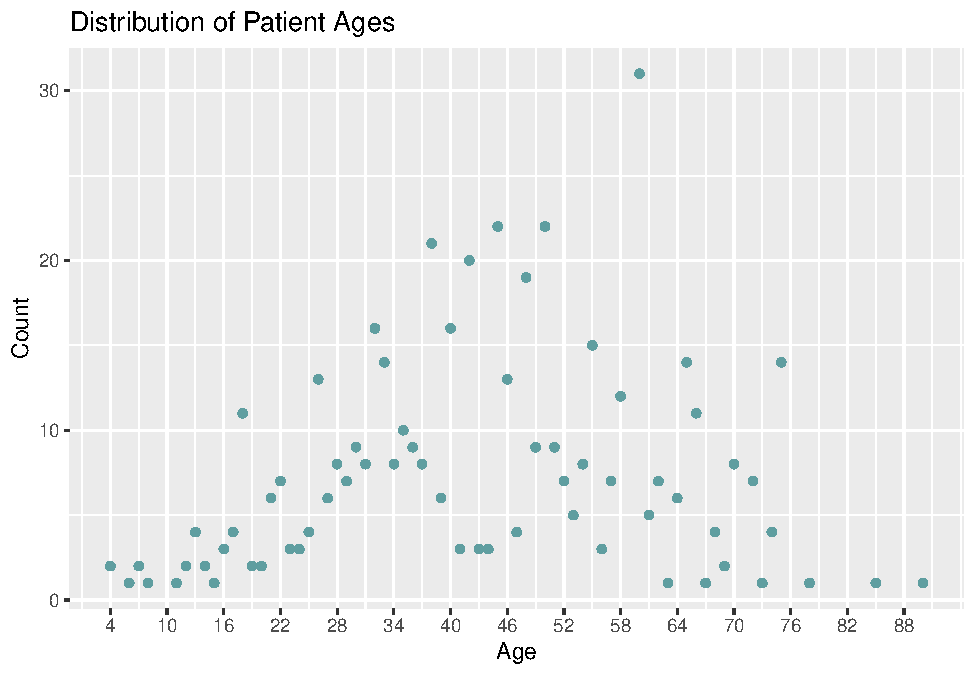
\includegraphics{LiverDisease_files/figure-latex/unnamed-chunk-11-1.pdf}
Now, we breakdown the distribution of ages to the presence or absence of
liver diseases. We notice a good spread of age group for both scenarios.

\begin{Shaded}
\begin{Highlighting}[]
\CommentTok{# Plotting distributions of ages based on liver diseases}
\NormalTok{training }\OperatorTok\StringTok{ }
\StringTok{  }\KeywordTok{ggplot}\NormalTok{(}\KeywordTok{aes}\NormalTok{(}\KeywordTok{as.numeric}\NormalTok{(}\KeywordTok{row.names}\NormalTok{(training)),Age, }\DataTypeTok{color=}\NormalTok{LiverDisease)) }\OperatorTok{+}
\StringTok{  }\KeywordTok{geom_point}\NormalTok{() }\OperatorTok{+}
\StringTok{  }\KeywordTok{labs}\NormalTok{(}\DataTypeTok{y=}\StringTok{"Age"}\NormalTok{, }\DataTypeTok{x =} \StringTok{"Number of patients"}\NormalTok{)}\OperatorTok{+}
\StringTok{  }\KeywordTok{facet_wrap}\NormalTok{( }\OperatorTok{~}\StringTok{ }\NormalTok{LiverDisease) }\OperatorTok{+}
\StringTok{  }\KeywordTok{ggtitle}\NormalTok{(}\StringTok{"Distribution of ages based on liver disease"}\NormalTok{)}
\end{Highlighting}
\end{Shaded}

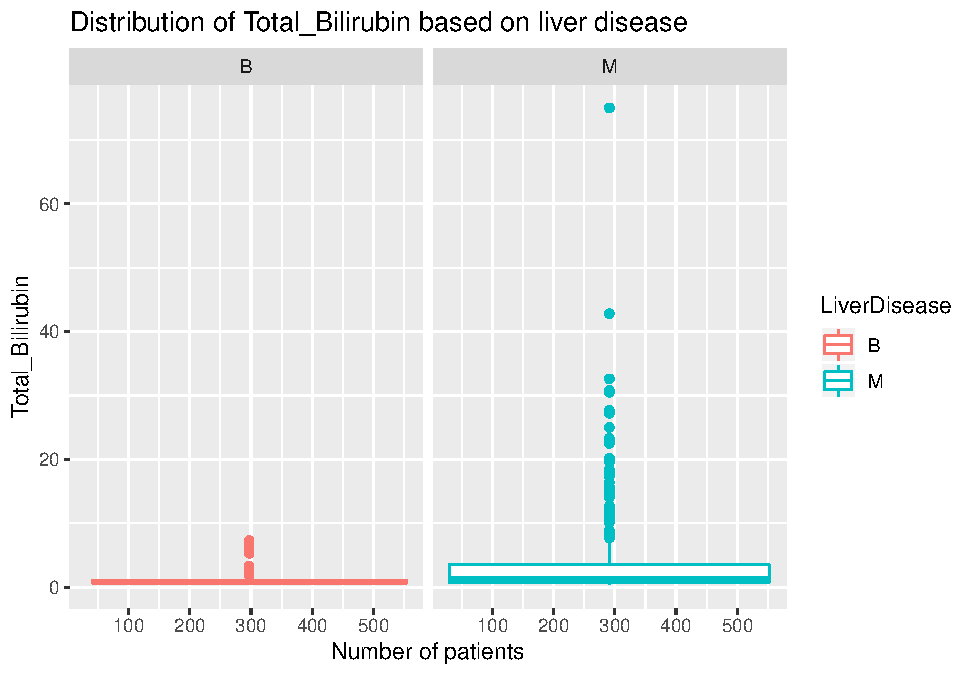
\includegraphics{LiverDisease_files/figure-latex/unnamed-chunk-12-1.pdf}

\subsection{Gender}

76\% of the patient records are of males. It would be good to have a
more and less equal distribution of records for both genders, although
we do not expect it to make any difference in the performance of our
models.

Both ``Gender'' and ``Age'' variables are not used to train the model.
These variables provide descriptive information.

\begin{Shaded}
\begin{Highlighting}[]
\CommentTok{# Getting summary of genders}
\KeywordTok{summary}\NormalTok{(training}\OperatorTok{$}\NormalTok{Gender)}
\end{Highlighting}
\end{Shaded}

\begin{verbatim}
## Female   Male 
##    123    400
\end{verbatim}

\textbackslash subsection\{Total\_Bilirubin and Direct\_Bilirubin\}
Bilirubin refers to any form of a yellowish pigment made in the liver
when red blood cells are broken down. The elevated levels of bilirubin
indicate that the liver is damaged. We find a similar trend with these
variables that levels of bilirubin are high for patients with liver
diseases.

\begin{Shaded}
\begin{Highlighting}[]
\CommentTok{# Plotting distributions of Total_Bilirubin based on liver diseases}
\NormalTok{training }\OperatorTok\StringTok{ }
\StringTok{  }\KeywordTok{ggplot}\NormalTok{(}\KeywordTok{aes}\NormalTok{(}\KeywordTok{as.numeric}\NormalTok{(}\KeywordTok{row.names}\NormalTok{(training)),Total_Bilirubin, }\DataTypeTok{color=}\NormalTok{LiverDisease)) }\OperatorTok{+}
\StringTok{  }\KeywordTok{geom_boxplot}\NormalTok{() }\OperatorTok{+}
\StringTok{  }\KeywordTok{labs}\NormalTok{(}\DataTypeTok{y=}\StringTok{"Total_Bilirubin"}\NormalTok{, }\DataTypeTok{x =} \StringTok{"Number of patients"}\NormalTok{)}\OperatorTok{+}
\StringTok{  }\KeywordTok{facet_wrap}\NormalTok{( }\OperatorTok{~}\StringTok{ }\NormalTok{LiverDisease) }\OperatorTok{+}
\StringTok{  }\KeywordTok{ggtitle}\NormalTok{(}\StringTok{"Distribution of Total_Bilirubin based on liver disease"}\NormalTok{)}
\end{Highlighting}
\end{Shaded}

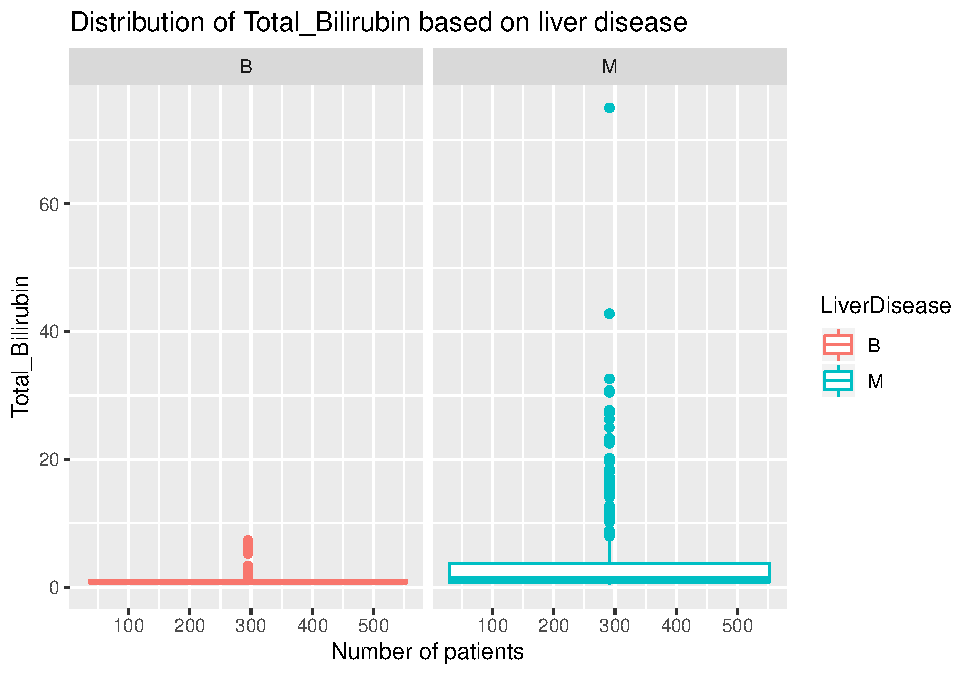
\includegraphics{LiverDisease_files/figure-latex/unnamed-chunk-14-1.pdf}

\begin{Shaded}
\begin{Highlighting}[]
\CommentTok{# Plotting distributions of Direct_Bilirubin based on liver disease}
\NormalTok{training }\OperatorTok\StringTok{ }
\StringTok{  }\KeywordTok{ggplot}\NormalTok{(}\KeywordTok{aes}\NormalTok{(}\KeywordTok{as.numeric}\NormalTok{(}\KeywordTok{row.names}\NormalTok{(training)),Direct_Bilirubin, }\DataTypeTok{color=}\NormalTok{LiverDisease)) }\OperatorTok{+}
\StringTok{  }\KeywordTok{geom_boxplot}\NormalTok{() }\OperatorTok{+}
\StringTok{  }\KeywordTok{labs}\NormalTok{(}\DataTypeTok{y=}\StringTok{"Direct_Bilirubin"}\NormalTok{, }\DataTypeTok{x =} \StringTok{"Number of patients"}\NormalTok{)}\OperatorTok{+}
\StringTok{  }\KeywordTok{facet_wrap}\NormalTok{( }\OperatorTok{~}\StringTok{ }\NormalTok{LiverDisease) }\OperatorTok{+}
\StringTok{  }\KeywordTok{ggtitle}\NormalTok{(}\StringTok{"Distribution of Direct_Bilirubin based on liver disease"}\NormalTok{)}
\end{Highlighting}
\end{Shaded}

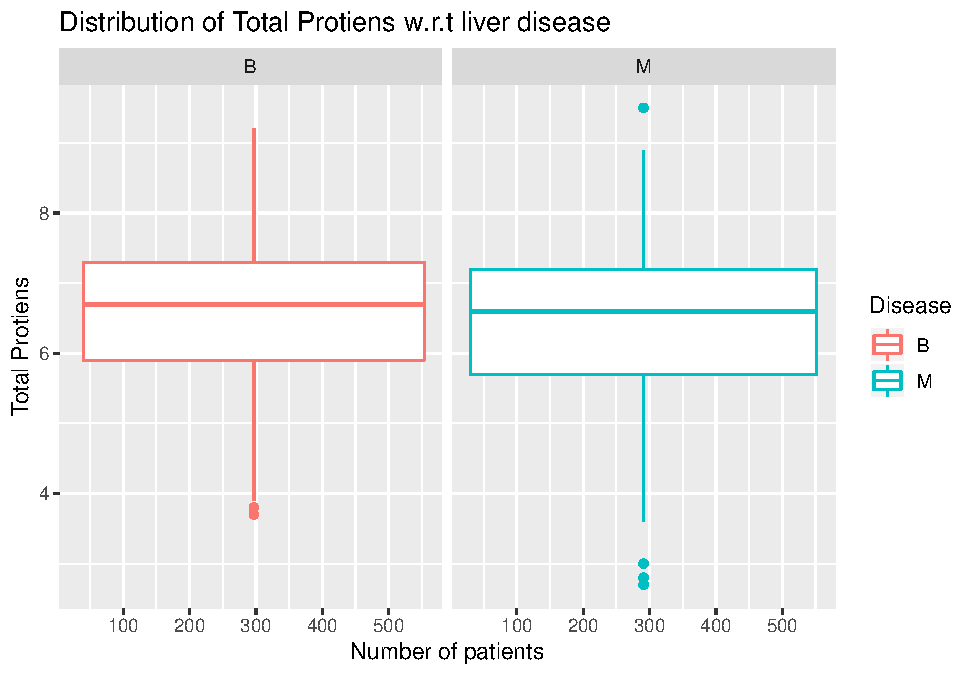
\includegraphics{LiverDisease_files/figure-latex/unnamed-chunk-15-1.pdf}

Now, we look at the correlations of bilirubins. We observe that both
bilirubins are weakly correlated with liver disease. However, both
bilirubins are highly correlated, and we can also use one of them to
train the model (if required).

\begin{Shaded}
\begin{Highlighting}[]
\CommentTok{# Making a subset of data}
\NormalTok{subset_train <-}\StringTok{ }\NormalTok{training[}\KeywordTok{c}\NormalTok{(}\StringTok{"Total_Bilirubin"}\NormalTok{,}\StringTok{"Direct_Bilirubin"}\NormalTok{,}\StringTok{"LiverDisease"}\NormalTok{)]}
\CommentTok{# Converting disease variable to numeric format}
\NormalTok{subset_train <-}\StringTok{ }\KeywordTok{transform}\NormalTok{(subset_train, }\DataTypeTok{LiverDisease=} \KeywordTok{ifelse}\NormalTok{(subset_train}\OperatorTok{$}\NormalTok{LiverDisease}\OperatorTok{==}\StringTok{"M"}\NormalTok{, }\DecValTok{1}\NormalTok{,}\DecValTok{0}\NormalTok{))}
\CommentTok{# Looking at the correlations}
\KeywordTok{cor}\NormalTok{(subset_train) }
\end{Highlighting}
\end{Shaded}

\begin{verbatim}
##                  Total_Bilirubin Direct_Bilirubin LiverDisease
## Total_Bilirubin        1.0000000        0.8655131    0.2165775
## Direct_Bilirubin       0.8655131        1.0000000    0.2429118
## LiverDisease           0.2165775        0.2429118    1.0000000
\end{verbatim}

\subsection{Alkaline Phosphotase}

Alkaline phosphatase (ALP) is an enzyme in a person's blood that helps
break down proteins. The elevated levels indicate that the liver has a
disease, and we notice a similar trend in our dataset.

\begin{Shaded}
\begin{Highlighting}[]
\CommentTok{# Plotting distributions of Alkaline Phosphotase based on liver diseases}
\NormalTok{training }\OperatorTok\StringTok{ }
\StringTok{  }\KeywordTok{ggplot}\NormalTok{(}\KeywordTok{aes}\NormalTok{(}\KeywordTok{as.numeric}\NormalTok{(}\KeywordTok{row.names}\NormalTok{(training)),Alkaline_Phosphotase, }\DataTypeTok{color=}\NormalTok{LiverDisease)) }\OperatorTok{+}
\StringTok{  }\KeywordTok{geom_boxplot}\NormalTok{() }\OperatorTok{+}
\StringTok{  }\KeywordTok{labs}\NormalTok{(}\DataTypeTok{y=}\StringTok{"Alkaline Phosphotase"}\NormalTok{, }\DataTypeTok{x =} \StringTok{"Number of patients"}\NormalTok{)}\OperatorTok{+}
\StringTok{  }\KeywordTok{facet_wrap}\NormalTok{( }\OperatorTok{~}\StringTok{ }\NormalTok{LiverDisease) }\OperatorTok{+}
\StringTok{  }\KeywordTok{ggtitle}\NormalTok{(}\StringTok{"Distribution of Alkaline Phosphotase based on liver disease"}\NormalTok{)}
\end{Highlighting}
\end{Shaded}

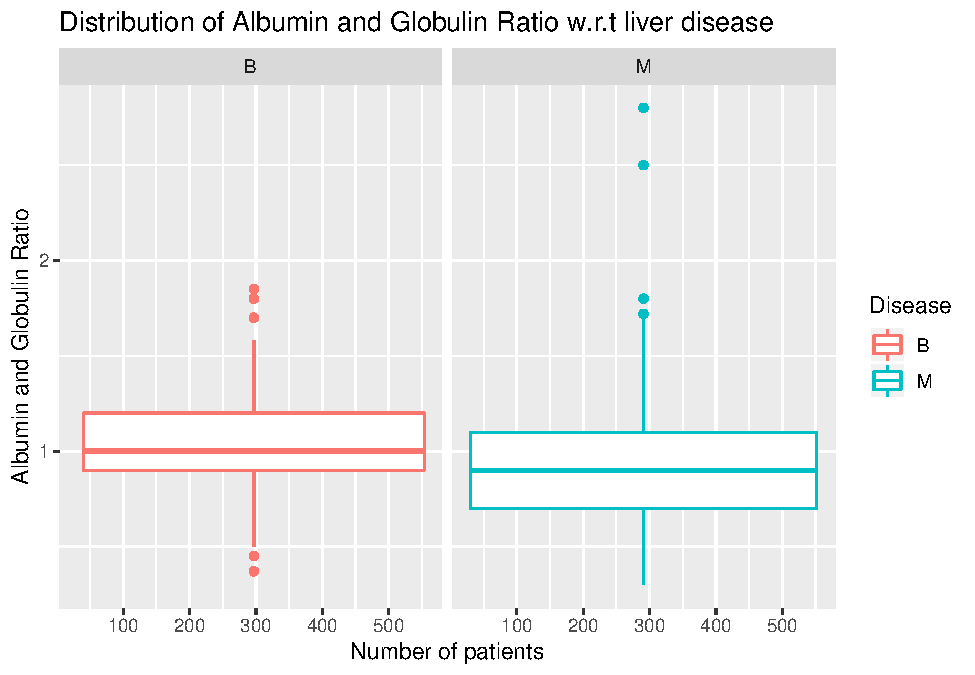
\includegraphics{LiverDisease_files/figure-latex/unnamed-chunk-17-1.pdf}

\textbackslash subsection\{Alamine\_Aminotransferase and
Aspartate\_Aminotransferase\} Aminotransferases are enzymes that are
important in the synthesis of amino acids, which form proteins. Alanine
aminotransferase (ALT) and Aspartate aminotransferase (AST) are found
primarily in the liver and kidney. High levels of ALT and AST are
expected for patients with liver diseases. We also notice slightly
elevated levels of these enzymes for patients with liver diseases in our
dataset.

\begin{Shaded}
\begin{Highlighting}[]
\CommentTok{# Plotting distributions of Alamine Aminotransferase based on liver diseases}
\NormalTok{training }\OperatorTok\StringTok{ }
\StringTok{  }\KeywordTok{ggplot}\NormalTok{(}\KeywordTok{aes}\NormalTok{(}\KeywordTok{as.numeric}\NormalTok{(}\KeywordTok{row.names}\NormalTok{(training)),Alamine_Aminotransferase, }\DataTypeTok{color=}\NormalTok{LiverDisease)) }\OperatorTok{+}
\StringTok{  }\KeywordTok{geom_boxplot}\NormalTok{() }\OperatorTok{+}
\StringTok{  }\KeywordTok{labs}\NormalTok{(}\DataTypeTok{y=}\StringTok{"Alamine Aminotransferase"}\NormalTok{, }\DataTypeTok{x =} \StringTok{"Number of patients"}\NormalTok{)}\OperatorTok{+}
\StringTok{  }\KeywordTok{facet_wrap}\NormalTok{( }\OperatorTok{~}\StringTok{ }\NormalTok{LiverDisease) }\OperatorTok{+}
\StringTok{  }\KeywordTok{ggtitle}\NormalTok{(}\StringTok{"Distribution of Alamine Aminotransferase based on liver disease"}\NormalTok{) }
\end{Highlighting}
\end{Shaded}

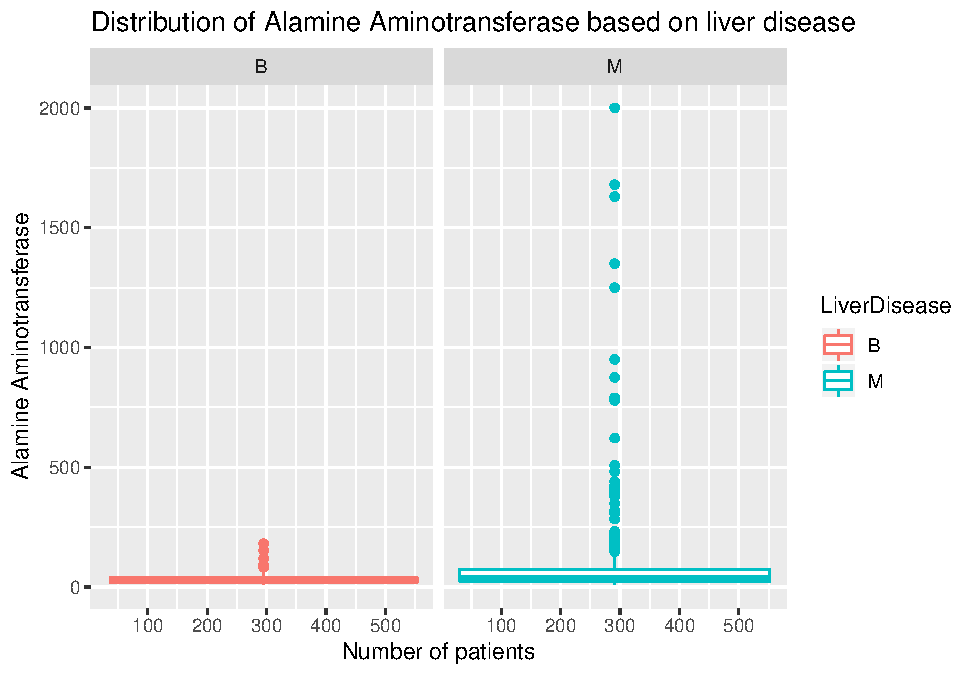
\includegraphics{LiverDisease_files/figure-latex/unnamed-chunk-18-1.pdf}

\begin{Shaded}
\begin{Highlighting}[]
\CommentTok{# Plotting distributions of Aspartate_Aminotransferase based on liver diseases}
\NormalTok{training }\OperatorTok\StringTok{ }
\StringTok{  }\KeywordTok{ggplot}\NormalTok{(}\KeywordTok{aes}\NormalTok{(}\KeywordTok{as.numeric}\NormalTok{(}\KeywordTok{row.names}\NormalTok{(training)),Aspartate_Aminotransferase, }\DataTypeTok{color=}\NormalTok{LiverDisease)) }\OperatorTok{+}
\StringTok{  }\KeywordTok{geom_boxplot}\NormalTok{() }\OperatorTok{+}
\StringTok{  }\KeywordTok{labs}\NormalTok{(}\DataTypeTok{y=}\StringTok{"Aspartate Aminotransferase"}\NormalTok{, }\DataTypeTok{x =} \StringTok{"Number of patients"}\NormalTok{)}\OperatorTok{+}
\StringTok{  }\KeywordTok{facet_wrap}\NormalTok{( }\OperatorTok{~}\StringTok{ }\NormalTok{LiverDisease) }\OperatorTok{+}
\StringTok{  }\KeywordTok{ggtitle}\NormalTok{(}\StringTok{"Distribution of Aspartate Aminotransferase based on liver disease"}\NormalTok{) }
\end{Highlighting}
\end{Shaded}

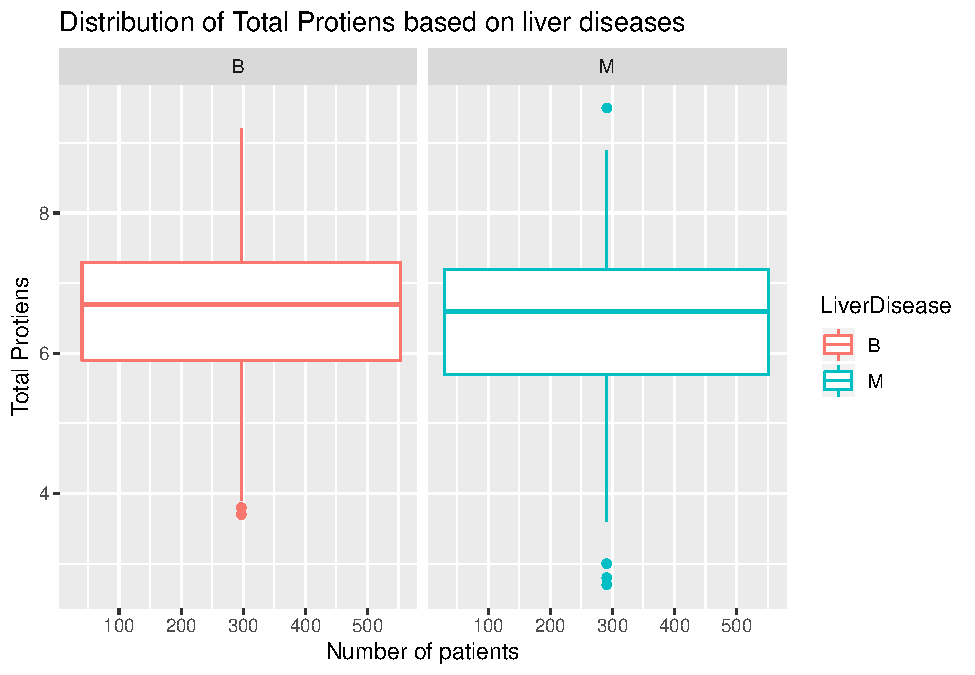
\includegraphics{LiverDisease_files/figure-latex/unnamed-chunk-19-1.pdf}

Contrary to bilirubins, there exists a weak correlation between both
aminotransferases.

\begin{Shaded}
\begin{Highlighting}[]
\CommentTok{# Making a subset of data}
\NormalTok{subset_train <-}\StringTok{ }\NormalTok{training[}\KeywordTok{c}\NormalTok{(}\StringTok{"Alkaline_Phosphotase"}\NormalTok{,}\StringTok{"Aspartate_Aminotransferase"}\NormalTok{,}\StringTok{"LiverDisease"}\NormalTok{)]}

\CommentTok{# Converting disease variable to numeric format}
\NormalTok{subset_train <-}\StringTok{ }\KeywordTok{transform}\NormalTok{(subset_train, }\DataTypeTok{LiverDisease=} \KeywordTok{ifelse}\NormalTok{(subset_train}\OperatorTok{$}\NormalTok{LiverDisease}\OperatorTok{==}\StringTok{"M"}\NormalTok{, }\DecValTok{1}\NormalTok{,}\DecValTok{0}\NormalTok{))}

\CommentTok{# Looking at the coorelations}
\KeywordTok{cor}\NormalTok{(subset_train) }
\end{Highlighting}
\end{Shaded}

\begin{verbatim}
##                            Alkaline_Phosphotase Aspartate_Aminotransferase
## Alkaline_Phosphotase                  1.0000000                  0.1644067
## Aspartate_Aminotransferase            0.1644067                  1.0000000
## LiverDisease                          0.1848371                  0.1524066
##                            LiverDisease
## Alkaline_Phosphotase          0.1848371
## Aspartate_Aminotransferase    0.1524066
## LiverDisease                  1.0000000
\end{verbatim}

\subsection{Total Protiens}

The total protein test measures the total amount of protein in your
body. The distributions indicate that this variable cannot be used to
diagnose liver disease. We do not see any pattern which we can use for
classification.

\begin{Shaded}
\begin{Highlighting}[]
\CommentTok{# Plotting distributions of Total Protiens based on liver diseases}
\NormalTok{training }\OperatorTok\StringTok{ }
\StringTok{  }\KeywordTok{ggplot}\NormalTok{(}\KeywordTok{aes}\NormalTok{(}\KeywordTok{as.numeric}\NormalTok{(}\KeywordTok{row.names}\NormalTok{(training)),Total_Protiens, }\DataTypeTok{color=}\NormalTok{LiverDisease)) }\OperatorTok{+}
\StringTok{  }\KeywordTok{geom_boxplot}\NormalTok{() }\OperatorTok{+}
\StringTok{  }\KeywordTok{labs}\NormalTok{(}\DataTypeTok{y=}\StringTok{"Total Protiens"}\NormalTok{, }\DataTypeTok{x =} \StringTok{"Number of patients"}\NormalTok{)}\OperatorTok{+}
\StringTok{  }\KeywordTok{facet_wrap}\NormalTok{( }\OperatorTok{~}\StringTok{ }\NormalTok{LiverDisease) }\OperatorTok{+}
\StringTok{  }\KeywordTok{ggtitle}\NormalTok{(}\StringTok{"Distribution of Total Protiens based on liver diseases"}\NormalTok{) }
\end{Highlighting}
\end{Shaded}

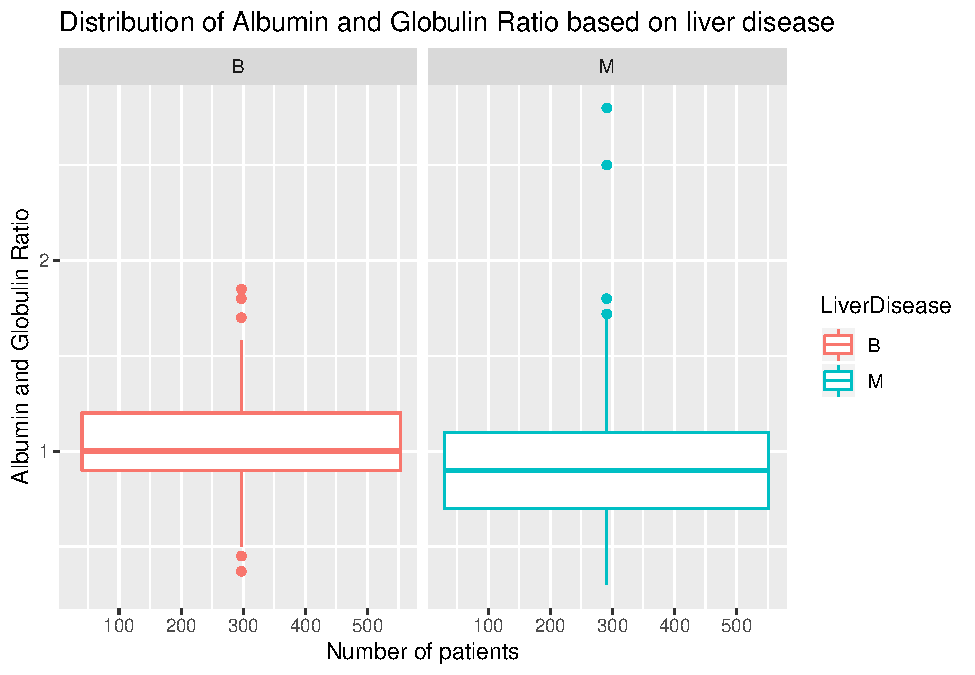
\includegraphics{LiverDisease_files/figure-latex/unnamed-chunk-21-1.pdf}

\subsection{Albumin}

Albumin is a protein made by the liver to keep fluid in the bloodstream.
The low levels of albumin indicate a problem with the liver, and we
notice a similar trend in our dataset.

\begin{Shaded}
\begin{Highlighting}[]
\CommentTok{# Plotting distributions of Albumin based on liver diseases}
\NormalTok{training }\OperatorTok\StringTok{ }
\StringTok{  }\KeywordTok{ggplot}\NormalTok{(}\KeywordTok{aes}\NormalTok{(}\KeywordTok{as.numeric}\NormalTok{(}\KeywordTok{row.names}\NormalTok{(training)),Albumin, }\DataTypeTok{color=}\NormalTok{LiverDisease)) }\OperatorTok{+}
\StringTok{  }\KeywordTok{geom_boxplot}\NormalTok{() }\OperatorTok{+}
\StringTok{  }\KeywordTok{labs}\NormalTok{(}\DataTypeTok{y=}\StringTok{"Albumin"}\NormalTok{, }\DataTypeTok{x =} \StringTok{"Number of patients"}\NormalTok{)}\OperatorTok{+}
\StringTok{  }\KeywordTok{facet_wrap}\NormalTok{( }\OperatorTok{~}\StringTok{ }\NormalTok{LiverDisease) }\OperatorTok{+}
\StringTok{  }\KeywordTok{ggtitle}\NormalTok{(}\StringTok{"Distribution of Albumin based on liver disease"}\NormalTok{) }
\end{Highlighting}
\end{Shaded}

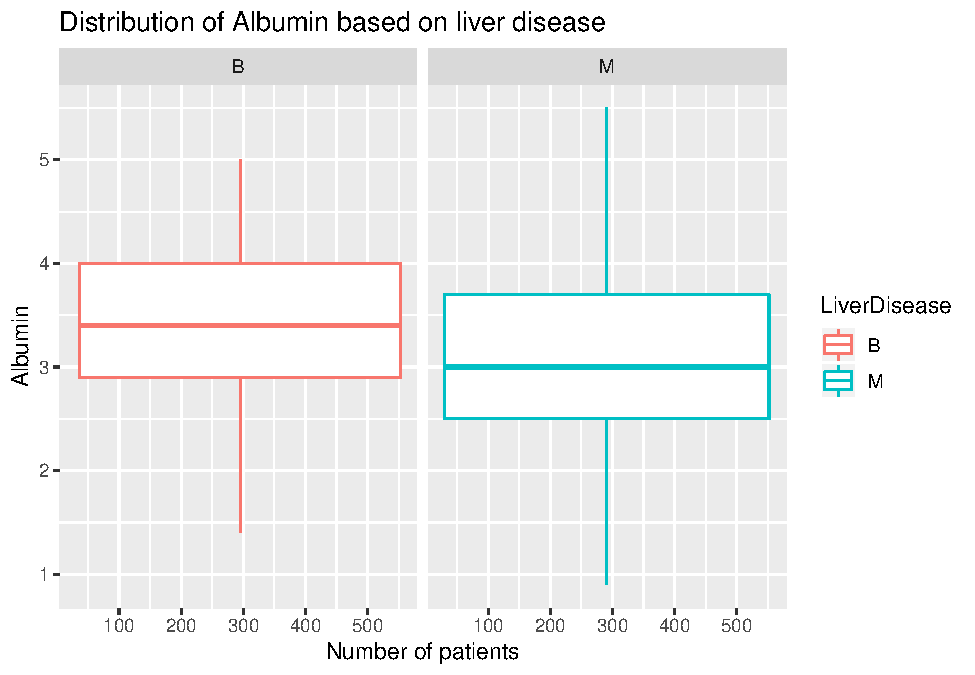
\includegraphics{LiverDisease_files/figure-latex/unnamed-chunk-22-1.pdf}

\textbackslash subsection\{Albumin\_and\_Globulin\_Ratio (AG)\} These
proteins are crucial for body growth, development, and health. They form
the structural part of most organs and makeup enzymes that regulate body
functions. The low ratios of AG refer to liver issues, and we notice the
same trend from distributions plot.

\begin{Shaded}
\begin{Highlighting}[]
\CommentTok{# Plotting distributions of Albumin based on liver diseases}
\NormalTok{training }\OperatorTok\StringTok{ }
\StringTok{  }\KeywordTok{ggplot}\NormalTok{(}\KeywordTok{aes}\NormalTok{(}\KeywordTok{as.numeric}\NormalTok{(}\KeywordTok{row.names}\NormalTok{(training)),Albumin_and_Globulin_Ratio, }\DataTypeTok{color=}\NormalTok{LiverDisease)) }\OperatorTok{+}
\StringTok{  }\KeywordTok{geom_boxplot}\NormalTok{() }\OperatorTok{+}
\StringTok{  }\KeywordTok{labs}\NormalTok{(}\DataTypeTok{y=}\StringTok{"Albumin and Globulin Ratio"}\NormalTok{, }\DataTypeTok{x =} \StringTok{"Number of patients"}\NormalTok{)}\OperatorTok{+}
\StringTok{  }\KeywordTok{facet_wrap}\NormalTok{( }\OperatorTok{~}\StringTok{ }\NormalTok{LiverDisease) }\OperatorTok{+}
\StringTok{  }\KeywordTok{ggtitle}\NormalTok{(}\StringTok{"Distribution of Albumin and Globulin Ratio based on liver disease"}\NormalTok{) }
\end{Highlighting}
\end{Shaded}

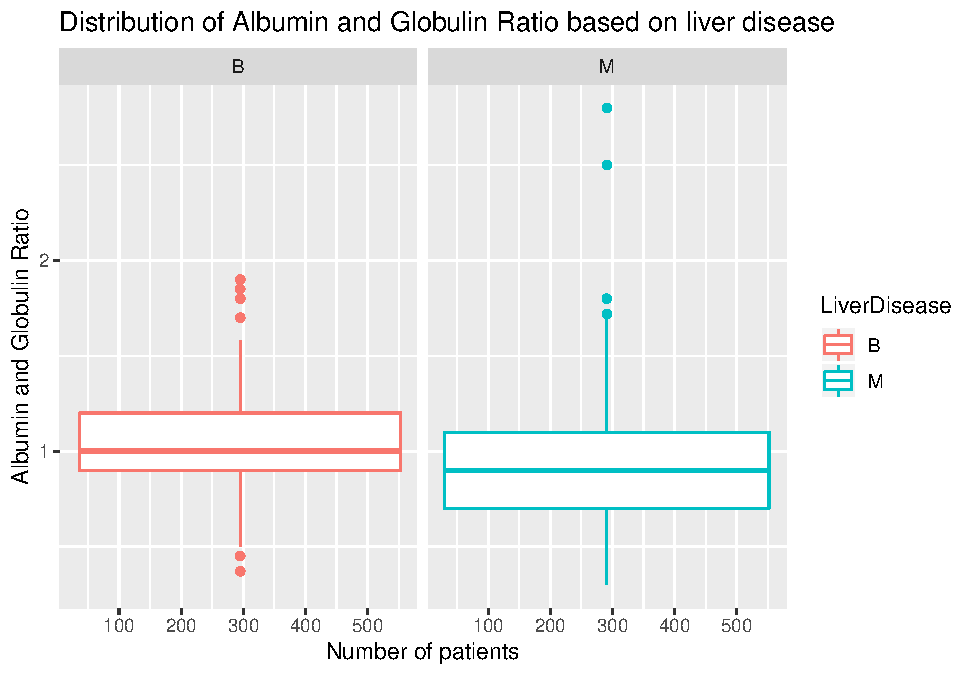
\includegraphics{LiverDisease_files/figure-latex/unnamed-chunk-23-1.pdf}

\section{Methods}
\label{sec:methods}

Based on the discussion in Section \ref{sec:dataanalysis}, we will not
use ``Age'' and ``Total Protein'' variables to train the machine
learning models. So, we remove these variables from both training and
validation datasets. Then, we predict the liver disease using all the
remaining variables of the dataset.

\begin{Shaded}
\begin{Highlighting}[]
\CommentTok{# Removing the variables 'Age' and 'Dataset' }
\NormalTok{training<-}\KeywordTok{within}\NormalTok{(training, }\KeywordTok{rm}\NormalTok{(Age,Total_Protiens))}
\NormalTok{validation<-}\KeywordTok{within}\NormalTok{(validation, }\KeywordTok{rm}\NormalTok{(Age,Total_Protiens))}
\end{Highlighting}
\end{Shaded}

For data pre-processing, we remove zero-variance predictors and then
center and scale all those remaining using the preProc argument. Feature
scaling is one of the most critical steps during the pre-processing of
data before creating a machine learning model. It can make a significant
difference between a weak machine learning model and a better one.

\subsection{Logistic Regression}

We use \emph{glm} method with cross-validation of 10 folds to train the
model.

\begin{Shaded}
\begin{Highlighting}[]
\CommentTok{# Defining a cross-validation (10 K folds )}
\NormalTok{control <-}\StringTok{ }\KeywordTok{trainControl}\NormalTok{(}\DataTypeTok{method =} \StringTok{"repeatedcv"}\NormalTok{, }\DataTypeTok{number =}\DecValTok{10}\NormalTok{,}\DataTypeTok{repeats =} \DecValTok{5}\NormalTok{)}

\CommentTok{# Train logistic regression model}
\NormalTok{train_glm <-}\StringTok{ }\KeywordTok{train}\NormalTok{(LiverDisease }\OperatorTok{~}\NormalTok{., }
                   \DataTypeTok{method =} \StringTok{"glm"}\NormalTok{,}
                   \DataTypeTok{preProc =} \KeywordTok{c}\NormalTok{(}\StringTok{"zv"}\NormalTok{,}\StringTok{"center"}\NormalTok{, }\StringTok{"scale"}\NormalTok{),}
                   \DataTypeTok{data =}\NormalTok{ training,}
                   \DataTypeTok{trControl=}\NormalTok{control)}

\CommentTok{# Showing the accuracy}
\KeywordTok{sprintf}\NormalTok{(}\StringTok{"The accuracy of GLM = %f"}\NormalTok{,train_glm}\OperatorTok{$}\NormalTok{results}\OperatorTok{$}\NormalTok{Accuracy)}
\end{Highlighting}
\end{Shaded}

\begin{verbatim}
## [1] "The accuracy of GLM = 0.702495"
\end{verbatim}

\begin{Shaded}
\begin{Highlighting}[]
\CommentTok{# Storing the results}
\NormalTok{model_results <-}\StringTok{ }\KeywordTok{data_frame}\NormalTok{(}\DataTypeTok{method =} \StringTok{"glm"}\NormalTok{, }\DataTypeTok{Accuracy =}\NormalTok{ train_glm}\OperatorTok{$}\NormalTok{results}\OperatorTok{$}\NormalTok{Accuracy)}
\end{Highlighting}
\end{Shaded}

\subsection{K-nearest neigbors (knn)}

We use \emph{knn} method with cross-validation of 10 folds to train the
model. We tune the model with several values of \emph{k}, ranging from 3
to 51, to optimize the performance.

\begin{Shaded}
\begin{Highlighting}[]
\KeywordTok{set.seed}\NormalTok{(}\DecValTok{1}\NormalTok{)}
\CommentTok{# Defining a cross validation (10 K folds )}
\NormalTok{control <-}\StringTok{ }\KeywordTok{trainControl}\NormalTok{(}\DataTypeTok{method =} \StringTok{"repeatedcv"}\NormalTok{, }\DataTypeTok{number =} \DecValTok{10}\NormalTok{, }\DataTypeTok{repeats=}\DecValTok{5}\NormalTok{)}

\CommentTok{# Train knn model}
\NormalTok{train_knn <-}\StringTok{ }\KeywordTok{train}\NormalTok{(LiverDisease}\OperatorTok{~}\StringTok{ }\NormalTok{.,}
                   \DataTypeTok{method =} \StringTok{"knn"}\NormalTok{, }
                   \DataTypeTok{preProc =} \KeywordTok{c}\NormalTok{(}\StringTok{"zv"}\NormalTok{,}\StringTok{"center"}\NormalTok{, }\StringTok{"scale"}\NormalTok{),}
                   \DataTypeTok{data =}\NormalTok{ training,}
                   \DataTypeTok{tuneGrid =} \KeywordTok{data.frame}\NormalTok{(}\DataTypeTok{k =} \KeywordTok{seq}\NormalTok{(}\DecValTok{3}\NormalTok{, }\DecValTok{51}\NormalTok{, }\DecValTok{2}\NormalTok{)),}
                   \DataTypeTok{trControl =}\NormalTok{ control)}

\CommentTok{# Plot the model and highlight the best result}
\KeywordTok{ggplot}\NormalTok{(train_knn, }\DataTypeTok{highlight =} \OtherTok{TRUE}\NormalTok{) }\OperatorTok{+}
\StringTok{  }\KeywordTok{ggtitle}\NormalTok{(}\KeywordTok{paste}\NormalTok{(}\StringTok{"The best accuracy = "}\NormalTok{,}\KeywordTok{round}\NormalTok{(}\KeywordTok{max}\NormalTok{(train_knn}\OperatorTok{$}\NormalTok{results}\OperatorTok{$}\NormalTok{Accuracy),}\DecValTok{3}\NormalTok{)))}
\end{Highlighting}
\end{Shaded}

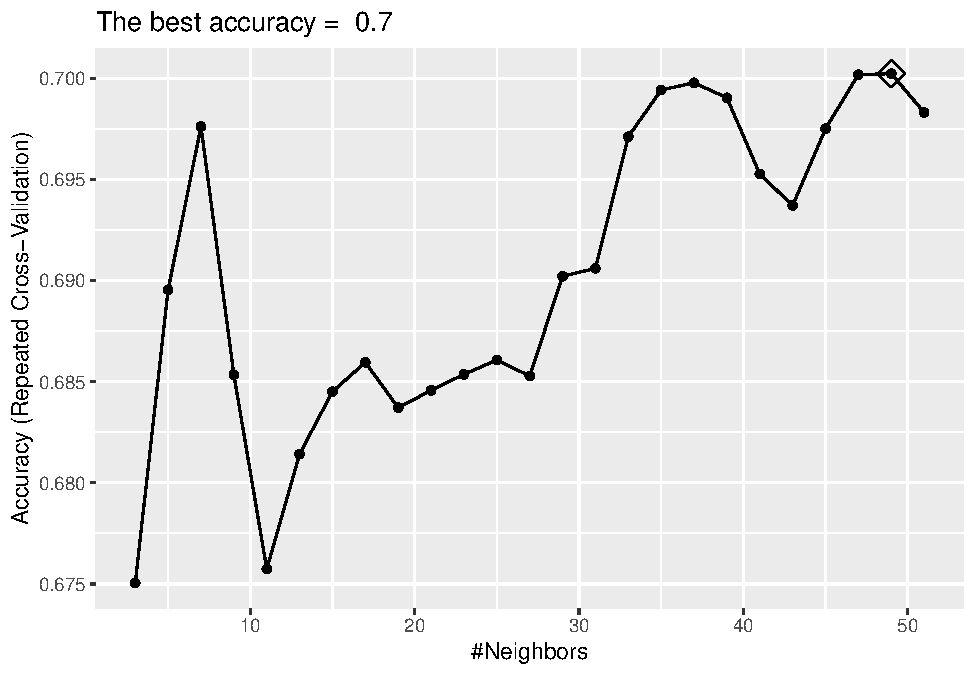
\includegraphics{LiverDisease_files/figure-latex/unnamed-chunk-26-1.pdf}

\begin{Shaded}
\begin{Highlighting}[]
\CommentTok{# Storing the results}
\NormalTok{model_results <-}\StringTok{ }\KeywordTok{bind_rows}\NormalTok{(model_results,}\KeywordTok{data_frame}\NormalTok{(}\DataTypeTok{method=}\StringTok{"knn"}\NormalTok{,  }
                                     \DataTypeTok{Accuracy =} \KeywordTok{max}\NormalTok{(train_knn}\OperatorTok{$}\NormalTok{results}\OperatorTok{$}\NormalTok{Accuracy) ))}
\end{Highlighting}
\end{Shaded}

\subsection{Local Regression}

We use \emph{loess} method with cross-validation of 10 folds to train
the model. We tune the \textbf{span} and \textbf{degree} parameters to
optimize the performance of the model.

\begin{Shaded}
\begin{Highlighting}[]
\KeywordTok{set.seed}\NormalTok{(}\DecValTok{1}\NormalTok{)}

\CommentTok{# Defining a cross validation (10 K folds )}
\NormalTok{control <-}\StringTok{ }\KeywordTok{trainControl}\NormalTok{(}\DataTypeTok{method =} \StringTok{"repeatedcv"}\NormalTok{, }\DataTypeTok{number =} \DecValTok{10}\NormalTok{, }\DataTypeTok{repeats=}\DecValTok{5}\NormalTok{)}

\CommentTok{# Define tuning parameters}
\NormalTok{tune_grid <-}\StringTok{ }\KeywordTok{expand.grid}\NormalTok{(}\DataTypeTok{span =} \KeywordTok{seq}\NormalTok{(}\FloatTok{0.15}\NormalTok{, }\FloatTok{0.65}\NormalTok{, }\DataTypeTok{len =} \DecValTok{15}\NormalTok{), }\DataTypeTok{degree =} \KeywordTok{seq}\NormalTok{(}\DecValTok{0}\NormalTok{,}\DecValTok{1}\NormalTok{,}\FloatTok{0.25}\NormalTok{))}

\CommentTok{# Train the model}
\NormalTok{train_loess <-}\StringTok{ }\KeywordTok{train}\NormalTok{(LiverDisease}\OperatorTok{~}\NormalTok{.,}
                   \DataTypeTok{method =} \StringTok{"gamLoess"}\NormalTok{,}
                   \DataTypeTok{preProc =} \KeywordTok{c}\NormalTok{(}\StringTok{"zv"}\NormalTok{,}\StringTok{"center"}\NormalTok{, }\StringTok{"scale"}\NormalTok{),}
                   \DataTypeTok{data =}\NormalTok{ training,}
                   \DataTypeTok{tuneGrid=}\NormalTok{ tune_grid, }
                   \DataTypeTok{trControl =}\NormalTok{ control)}

\CommentTok{# Plot the model and highlight the best result}
\KeywordTok{ggplot}\NormalTok{(train_loess, }\DataTypeTok{highlight =} \OtherTok{TRUE}\NormalTok{) }\OperatorTok{+}
\StringTok{  }\KeywordTok{ggtitle}\NormalTok{(}\KeywordTok{paste}\NormalTok{(}\StringTok{"The best accuracy = "}\NormalTok{,}\KeywordTok{round}\NormalTok{(}\KeywordTok{max}\NormalTok{(train_loess}\OperatorTok{$}\NormalTok{results}\OperatorTok{$}\NormalTok{Accuracy),}\DecValTok{3}\NormalTok{)))}
\end{Highlighting}
\end{Shaded}

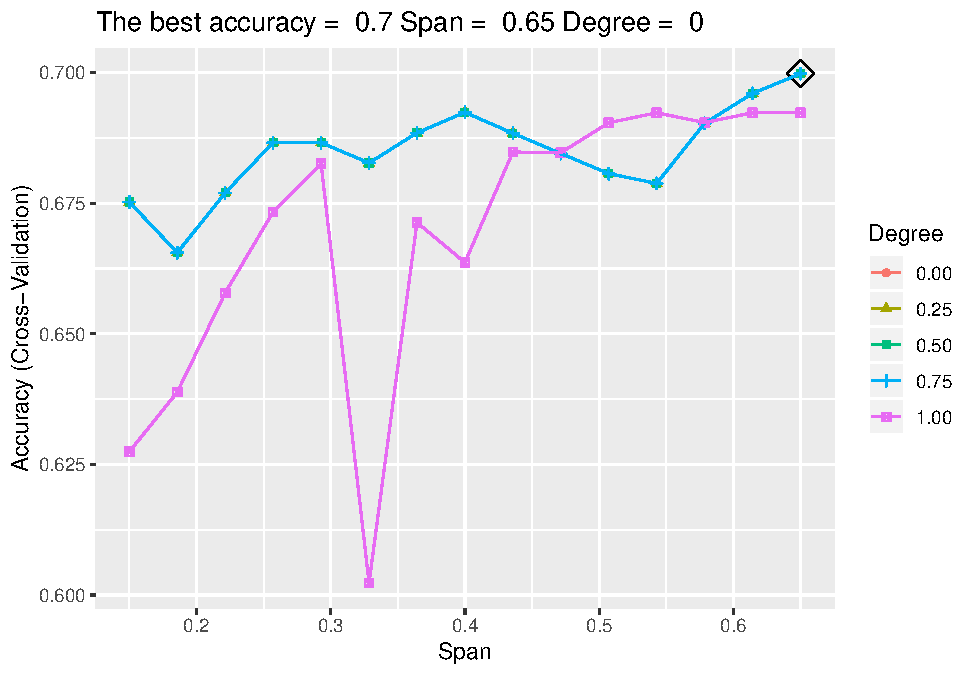
\includegraphics{LiverDisease_files/figure-latex/unnamed-chunk-27-1.pdf}

\begin{Shaded}
\begin{Highlighting}[]
\CommentTok{# Storing the results}
\NormalTok{model_results <-}\StringTok{ }\KeywordTok{bind_rows}\NormalTok{(model_results,}\KeywordTok{data_frame}\NormalTok{(}\DataTypeTok{method=}\StringTok{"loess"}\NormalTok{,  }
                                     \DataTypeTok{Accuracy =} \KeywordTok{max}\NormalTok{(train_loess}\OperatorTok{$}\NormalTok{results}\OperatorTok{$}\NormalTok{Accuracy) ))}
\end{Highlighting}
\end{Shaded}

\subsection{Partial Least Squares (PLS)}

We use \emph{pls} method with cross-validation of 10 folds to train the
model. We tune the \textbf{ncomp} parameter to optimize the performance
of the model.

\begin{Shaded}
\begin{Highlighting}[]
\KeywordTok{set.seed}\NormalTok{(}\DecValTok{1}\NormalTok{)}

\CommentTok{# Define tuning parameters}
\NormalTok{tune_grid <-}\StringTok{ }\KeywordTok{expand.grid}\NormalTok{(}\DataTypeTok{ncomp =} \KeywordTok{seq}\NormalTok{(}\DecValTok{1}\NormalTok{,}\DecValTok{5}\NormalTok{, }\DataTypeTok{len =} \DecValTok{10}\NormalTok{))}

\CommentTok{# Defining a cross validation (10 K folds )}
\NormalTok{control <-}\StringTok{ }\KeywordTok{trainControl}\NormalTok{(}\DataTypeTok{method =} \StringTok{"repeatedcv"}\NormalTok{, }\DataTypeTok{number =} \DecValTok{10}\NormalTok{, }\DataTypeTok{repeats=}\DecValTok{5}\NormalTok{)}

\CommentTok{# Train the model}
\NormalTok{train_pls <-}\StringTok{ }\KeywordTok{train}\NormalTok{(LiverDisease}\OperatorTok{~}\NormalTok{.,}
                   \DataTypeTok{method =} \StringTok{"pls"}\NormalTok{,}
                   \DataTypeTok{preProc =} \KeywordTok{c}\NormalTok{(}\StringTok{"zv"}\NormalTok{,}\StringTok{"center"}\NormalTok{, }\StringTok{"scale"}\NormalTok{),}
                   \DataTypeTok{data =}\NormalTok{ training,}
                   \DataTypeTok{tuneGrid=}\NormalTok{ tune_grid,}
                   \DataTypeTok{trControl =}\NormalTok{ control)}

\CommentTok{# Plot the model and highlight the best result}
\KeywordTok{ggplot}\NormalTok{(train_pls, }\DataTypeTok{highlight =} \OtherTok{TRUE}\NormalTok{) }\OperatorTok{+}
\StringTok{  }\KeywordTok{ggtitle}\NormalTok{(}\KeywordTok{paste}\NormalTok{(}\StringTok{"The best accuracy = "}\NormalTok{,}\KeywordTok{round}\NormalTok{(}\KeywordTok{max}\NormalTok{(train_pls}\OperatorTok{$}\NormalTok{results}\OperatorTok{$}\NormalTok{Accuracy),}\DecValTok{3}\NormalTok{)))}
\end{Highlighting}
\end{Shaded}

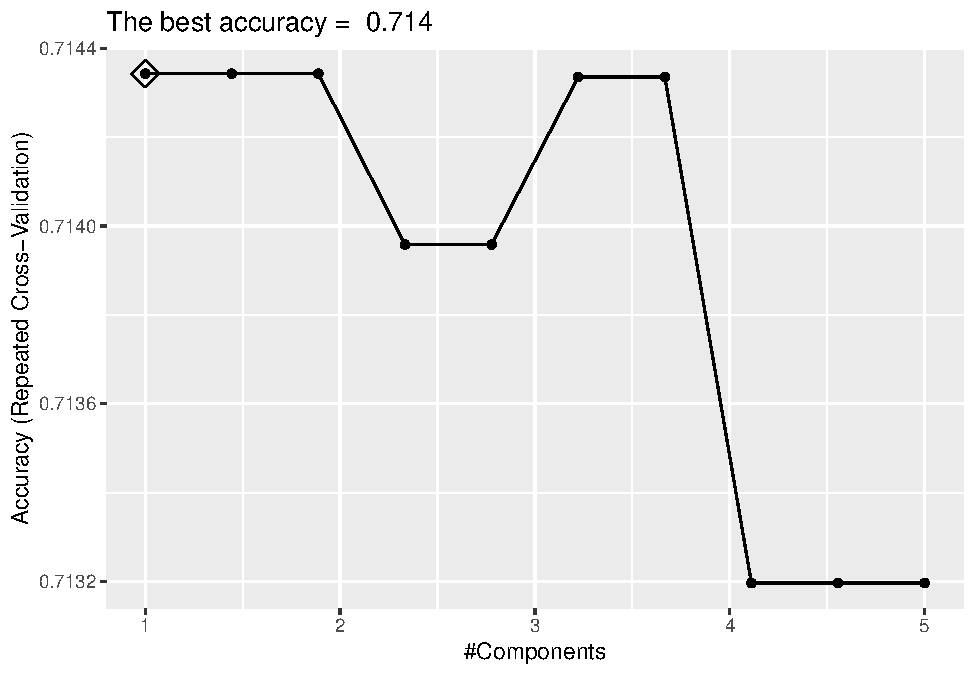
\includegraphics{LiverDisease_files/figure-latex/unnamed-chunk-28-1.pdf}

\begin{Shaded}
\begin{Highlighting}[]
\CommentTok{# Storing the results}
\NormalTok{model_results <-}\StringTok{ }\KeywordTok{bind_rows}\NormalTok{(model_results,}\KeywordTok{data_frame}\NormalTok{(}\DataTypeTok{method=}\StringTok{"pls"}\NormalTok{,  }
                                     \DataTypeTok{Accuracy =} \KeywordTok{max}\NormalTok{(train_pls}\OperatorTok{$}\NormalTok{results}\OperatorTok{$}\NormalTok{Accuracy) ))}
\end{Highlighting}
\end{Shaded}

\subsection{Linear Discriminant Analysis (LDA)}

The \emph{lda} is a statistical classifier, and we use this method with
cross-validation of 10 folds for training. There is no parameter to tune
for this model.

\begin{Shaded}
\begin{Highlighting}[]
\KeywordTok{set.seed}\NormalTok{(}\DecValTok{1}\NormalTok{)}
\CommentTok{# Defining a cross validation (10 K folds )}
\NormalTok{control <-}\StringTok{ }\KeywordTok{trainControl}\NormalTok{(}\DataTypeTok{method =} \StringTok{"repeatedcv"}\NormalTok{, }\DataTypeTok{number=}\DecValTok{10}\NormalTok{, }\DataTypeTok{repeats=}\DecValTok{5}\NormalTok{)}

\CommentTok{# Train the model}
\NormalTok{train_lda <-}\StringTok{ }\KeywordTok{train}\NormalTok{(LiverDisease}\OperatorTok{~}\NormalTok{., }
                   \DataTypeTok{method =} \StringTok{"lda"}\NormalTok{,}
                   \DataTypeTok{preProc =} \KeywordTok{c}\NormalTok{(}\StringTok{"zv"}\NormalTok{,}\StringTok{"center"}\NormalTok{, }\StringTok{"scale"}\NormalTok{),}
                   \DataTypeTok{data =}\NormalTok{ training,}
                   \DataTypeTok{trControl =}\NormalTok{ control)}

\KeywordTok{sprintf}\NormalTok{(}\StringTok{"The accuracy of lda = %f"}\NormalTok{,}\KeywordTok{max}\NormalTok{(train_lda}\OperatorTok{$}\NormalTok{results}\OperatorTok{$}\NormalTok{Accuracy))}
\end{Highlighting}
\end{Shaded}

\begin{verbatim}
## [1] "The accuracy of lda = 0.710134"
\end{verbatim}

\begin{Shaded}
\begin{Highlighting}[]
\CommentTok{# Storing the results}
\NormalTok{model_results <-}\StringTok{ }\KeywordTok{bind_rows}\NormalTok{(model_results,}\KeywordTok{data_frame}\NormalTok{(}\DataTypeTok{method=}\StringTok{"lda"}\NormalTok{,  }
                                     \DataTypeTok{Accuracy =} \KeywordTok{max}\NormalTok{(train_lda}\OperatorTok{$}\NormalTok{results}\OperatorTok{$}\NormalTok{Accuracy) ))}
\end{Highlighting}
\end{Shaded}

\subsection{Quadratic Discriminant Analysis (QDA)}

The \emph{qda} is a statistical classifier, and we use the method with
cross-validation of 10 folds for training. There is no parameter to tune
for this model.

\begin{Shaded}
\begin{Highlighting}[]
\KeywordTok{set.seed}\NormalTok{(}\DecValTok{1}\NormalTok{)}
\CommentTok{# Defining a cross validation (10 K folds )}
\NormalTok{control <-}\StringTok{ }\KeywordTok{trainControl}\NormalTok{(}\DataTypeTok{method =} \StringTok{"repeatedcv"}\NormalTok{, }\DataTypeTok{number=}\DecValTok{10}\NormalTok{, }\DataTypeTok{repeats=}\DecValTok{5}\NormalTok{)}

\CommentTok{# Train the model}
\NormalTok{train_qda <-}\StringTok{ }\KeywordTok{train}\NormalTok{(LiverDisease}\OperatorTok{~}\NormalTok{.,}
                   \DataTypeTok{method =} \StringTok{"qda"}\NormalTok{,}
                   \DataTypeTok{preProc =} \KeywordTok{c}\NormalTok{(}\StringTok{"zv"}\NormalTok{,}\StringTok{"center"}\NormalTok{, }\StringTok{"scale"}\NormalTok{),}
                   \DataTypeTok{data =}\NormalTok{ training,}
                   \DataTypeTok{trControl =}\NormalTok{ control)}

\KeywordTok{sprintf}\NormalTok{(}\StringTok{"The accuracy of qda = %f"}\NormalTok{,}\KeywordTok{max}\NormalTok{(train_qda}\OperatorTok{$}\NormalTok{results}\OperatorTok{$}\NormalTok{Accuracy))}
\end{Highlighting}
\end{Shaded}

\begin{verbatim}
## [1] "The accuracy of qda = 0.557171"
\end{verbatim}

\begin{Shaded}
\begin{Highlighting}[]
\CommentTok{# Storing the results}
\NormalTok{model_results <-}\StringTok{ }\KeywordTok{bind_rows}\NormalTok{(model_results,}\KeywordTok{data_frame}\NormalTok{(}\DataTypeTok{method=}\StringTok{"qda"}\NormalTok{,  }
                                     \DataTypeTok{Accuracy =} \KeywordTok{max}\NormalTok{(train_qda}\OperatorTok{$}\NormalTok{results}\OperatorTok{$}\NormalTok{Accuracy) ))}
\end{Highlighting}
\end{Shaded}

\subsection{Decision Tress}

We use \emph{raprt} method with cross-validation of 10 folds for
training. We tune the \emph{cp} parameter to optimize the performance of
the model.

\begin{Shaded}
\begin{Highlighting}[]
\KeywordTok{set.seed}\NormalTok{(}\DecValTok{1}\NormalTok{)}

\CommentTok{# Defining a cross validation (10 K folds )}
\NormalTok{control <-}\StringTok{ }\KeywordTok{trainControl}\NormalTok{(}\DataTypeTok{method =} \StringTok{"repeatedcv"}\NormalTok{, }\DataTypeTok{number =} \DecValTok{10}\NormalTok{, }\DataTypeTok{repeats=}\DecValTok{5}\NormalTok{)}

\CommentTok{# Train the model}
\NormalTok{train_rpart <-}\StringTok{ }\KeywordTok{train}\NormalTok{(LiverDisease}\OperatorTok{~}\NormalTok{., }
                     \DataTypeTok{method =} \StringTok{"rpart"}\NormalTok{,}
                     \DataTypeTok{preProc =} \KeywordTok{c}\NormalTok{(}\StringTok{"zv"}\NormalTok{,}\StringTok{"center"}\NormalTok{, }\StringTok{"scale"}\NormalTok{),}
                     \DataTypeTok{data =}\NormalTok{ training,}
                     \DataTypeTok{trControl =}\NormalTok{ control,}
                     \DataTypeTok{tuneGrid =} \KeywordTok{data.frame}\NormalTok{(}\DataTypeTok{cp =} \KeywordTok{seq}\NormalTok{(}\DecValTok{0}\NormalTok{, }\FloatTok{0.08}\NormalTok{, }\DataTypeTok{len =} \DecValTok{10}\NormalTok{)))}

\CommentTok{# Plot the model and highlight the best result}
\KeywordTok{ggplot}\NormalTok{(train_rpart, }\DataTypeTok{highlight =} \OtherTok{TRUE}\NormalTok{) }\OperatorTok{+}
\StringTok{  }\KeywordTok{ggtitle}\NormalTok{(}\KeywordTok{paste}\NormalTok{(}\StringTok{"The best accuracy = "}\NormalTok{,}\KeywordTok{round}\NormalTok{(}\KeywordTok{max}\NormalTok{(train_rpart}\OperatorTok{$}\NormalTok{results}\OperatorTok{$}\NormalTok{Accuracy),}\DecValTok{3}\NormalTok{)))}
\end{Highlighting}
\end{Shaded}

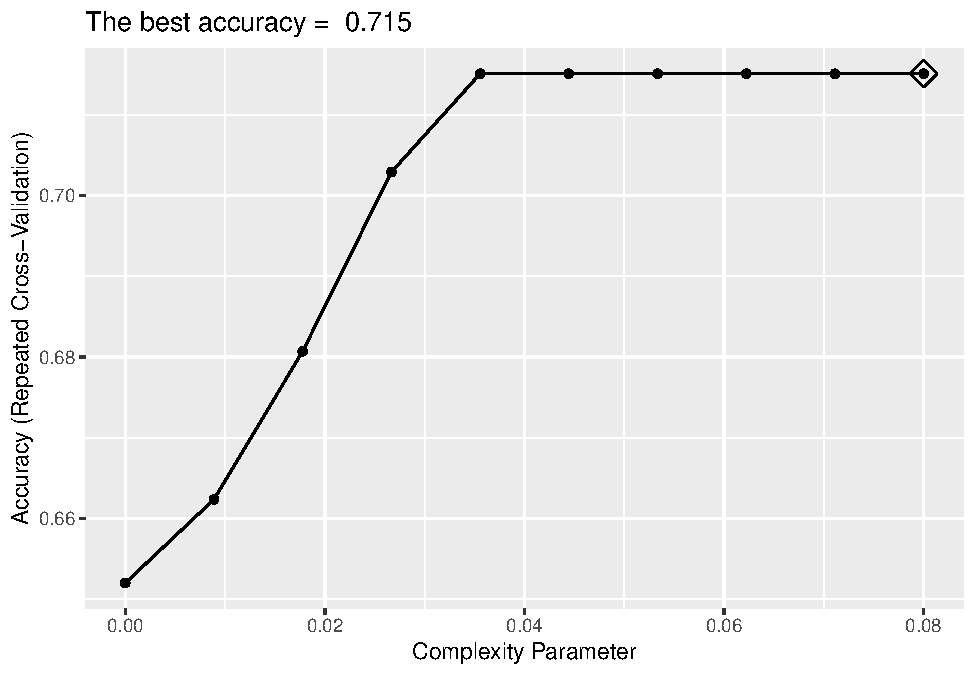
\includegraphics{LiverDisease_files/figure-latex/unnamed-chunk-31-1.pdf}

\begin{Shaded}
\begin{Highlighting}[]
\CommentTok{# Storing the results}
\NormalTok{model_results <-}\StringTok{ }\KeywordTok{bind_rows}\NormalTok{(model_results,}\KeywordTok{data_frame}\NormalTok{(}\DataTypeTok{method=}\StringTok{"rpart"}\NormalTok{,  }
                                     \DataTypeTok{Accuracy =} \KeywordTok{max}\NormalTok{(train_rpart}\OperatorTok{$}\NormalTok{results}\OperatorTok{$}\NormalTok{Accuracy) ))}
\end{Highlighting}
\end{Shaded}

\subsection{Random Forests}

We use \emph{rf} method with cross-validation of 10 folds for training.
We tune the \emph{mtry} parameter to optimize the performance of the
model.

\begin{Shaded}
\begin{Highlighting}[]
\KeywordTok{set.seed}\NormalTok{(}\DecValTok{1}\NormalTok{)}

\CommentTok{# Defining a cross validation (10 K folds )}
\NormalTok{control <-}\StringTok{ }\KeywordTok{trainControl}\NormalTok{(}\DataTypeTok{method =} \StringTok{"repeatedcv"}\NormalTok{, }\DataTypeTok{number =} \DecValTok{10}\NormalTok{, }\DataTypeTok{repeats=}\DecValTok{5}\NormalTok{)}

\CommentTok{# Train the model}
\NormalTok{train_rf <-}\StringTok{ }\KeywordTok{train}\NormalTok{(LiverDisease}\OperatorTok{~}\NormalTok{.,}
                     \DataTypeTok{method =} \StringTok{"rf"}\NormalTok{,}
                     \DataTypeTok{preProc =} \KeywordTok{c}\NormalTok{(}\StringTok{"zv"}\NormalTok{,}\StringTok{"center"}\NormalTok{, }\StringTok{"scale"}\NormalTok{),}
                     \DataTypeTok{data =}\NormalTok{ training,}
                     \DataTypeTok{trControl =}\NormalTok{ control,}
                     \DataTypeTok{tuneGrid =} \KeywordTok{data.frame}\NormalTok{(}\DataTypeTok{mtry=}\KeywordTok{seq}\NormalTok{(}\DecValTok{1}\NormalTok{,}\DecValTok{7}\NormalTok{)),}
                     \DataTypeTok{ntree=}\DecValTok{100}\NormalTok{)}

\CommentTok{# Plot the model and highlight the best result}
\KeywordTok{ggplot}\NormalTok{(train_rf, }\DataTypeTok{highlight =} \OtherTok{TRUE}\NormalTok{) }\OperatorTok{+}
\StringTok{  }\KeywordTok{ggtitle}\NormalTok{(}\KeywordTok{paste}\NormalTok{(}\StringTok{"The best accuracy = "}\NormalTok{,}\KeywordTok{round}\NormalTok{(}\KeywordTok{max}\NormalTok{(train_rf}\OperatorTok{$}\NormalTok{results}\OperatorTok{$}\NormalTok{Accuracy),}\DecValTok{3}\NormalTok{)))}
\end{Highlighting}
\end{Shaded}

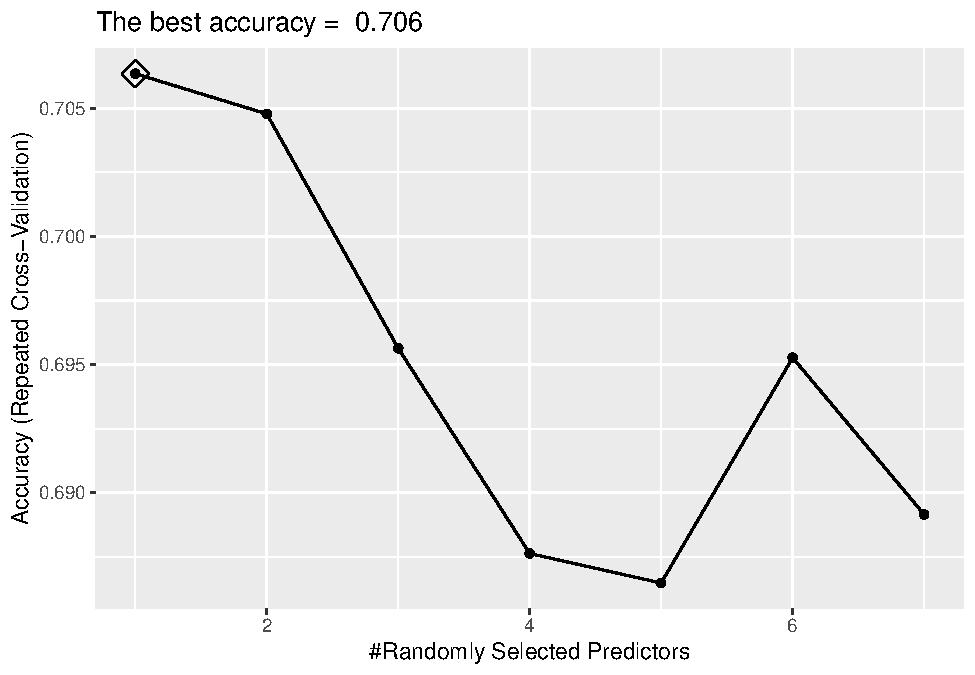
\includegraphics{LiverDisease_files/figure-latex/unnamed-chunk-32-1.pdf}

\begin{Shaded}
\begin{Highlighting}[]
\CommentTok{# Storing the results}
\NormalTok{model_results <-}\StringTok{ }\KeywordTok{bind_rows}\NormalTok{(model_results,}\KeywordTok{data_frame}\NormalTok{(}\DataTypeTok{method=}\StringTok{"rf"}\NormalTok{,  }
                                     \DataTypeTok{Accuracy =} \KeywordTok{max}\NormalTok{(train_rf}\OperatorTok{$}\NormalTok{results}\OperatorTok{$}\NormalTok{Accuracy) ))}
\end{Highlighting}
\end{Shaded}

\subsection{Support Vector Machine}

We use support vector machine with cross-validation of 10 folds for
training. We tune the \emph{tau} parameter to optimize the performance
of the model.

\begin{Shaded}
\begin{Highlighting}[]
\KeywordTok{set.seed}\NormalTok{(}\DecValTok{1}\NormalTok{)}

\CommentTok{# Defining a cross validation (10 K folds )}
\NormalTok{control <-}\StringTok{ }\KeywordTok{trainControl}\NormalTok{(}\DataTypeTok{method =} \StringTok{"repeatedcv"}\NormalTok{, }\DataTypeTok{number =} \DecValTok{10}\NormalTok{, }\DataTypeTok{repeats =} \DecValTok{5}\NormalTok{)}

\CommentTok{# Train the model}
\NormalTok{train_svm <-}\StringTok{ }\KeywordTok{train}\NormalTok{(LiverDisease}\OperatorTok{~}\NormalTok{.,}
                   \DataTypeTok{preProc =} \KeywordTok{c}\NormalTok{(}\StringTok{"zv"}\NormalTok{,}\StringTok{"center"}\NormalTok{, }\StringTok{"scale"}\NormalTok{),}
                   \DataTypeTok{data =}\NormalTok{ training,}
                   \DataTypeTok{method =} \StringTok{"svmLinear"}\NormalTok{,}
                   \DataTypeTok{tune_grid=} \KeywordTok{data.frame}\NormalTok{(}\DataTypeTok{tau=}\KeywordTok{seq}\NormalTok{(}\DecValTok{1}\NormalTok{,}\DecValTok{10}\NormalTok{)),}
                   \DataTypeTok{trControl =}\NormalTok{ control)}

\KeywordTok{sprintf}\NormalTok{(}\StringTok{"The accuracy of svm = %f"}\NormalTok{,}\KeywordTok{max}\NormalTok{(train_svm}\OperatorTok{$}\NormalTok{results}\OperatorTok{$}\NormalTok{Accuracy))}
\end{Highlighting}
\end{Shaded}

\begin{verbatim}
## [1] "The accuracy of svm = 0.715098"
\end{verbatim}

\begin{Shaded}
\begin{Highlighting}[]
\CommentTok{# Storing the results}
\NormalTok{model_results <-}\StringTok{ }\KeywordTok{bind_rows}\NormalTok{(model_results,}\KeywordTok{data_frame}\NormalTok{(}\DataTypeTok{method=}\StringTok{"svm"}\NormalTok{,  }
                                     \DataTypeTok{Accuracy =} \KeywordTok{max}\NormalTok{(train_svm}\OperatorTok{$}\NormalTok{results}\OperatorTok{$}\NormalTok{Accuracy) ))}
\end{Highlighting}
\end{Shaded}

\subsection{Adaptive Boosting (Adaboost)}

AdaBoost is a machine learning meta-algorithm for classification. We
train the model with cross-validation of 10 folds.

\begin{Shaded}
\begin{Highlighting}[]
\KeywordTok{set.seed}\NormalTok{(}\DecValTok{1}\NormalTok{)}

\CommentTok{# Defining a cross validation (10 K folds )}
\NormalTok{control <-}\StringTok{ }\KeywordTok{trainControl}\NormalTok{(}\DataTypeTok{method =} \StringTok{"repeatedcv"}\NormalTok{, }\DataTypeTok{number =} \DecValTok{10}\NormalTok{, }\DataTypeTok{repeats =} \DecValTok{5}\NormalTok{)}

\CommentTok{# Tuning the model}
\NormalTok{tune_grid  =}\StringTok{ }\KeywordTok{expand.grid}\NormalTok{(}\DataTypeTok{method =} \KeywordTok{c}\NormalTok{(}\StringTok{"Adaboost.M1"}\NormalTok{, }\StringTok{"Real adaboost"}\NormalTok{))}
 
\NormalTok{train_ada <-}\StringTok{ }\KeywordTok{train}\NormalTok{(LiverDisease}\OperatorTok{~}\NormalTok{.,}
                   \DataTypeTok{preProc =} \KeywordTok{c}\NormalTok{(}\StringTok{"zv"}\NormalTok{,}\StringTok{"center"}\NormalTok{, }\StringTok{"scale"}\NormalTok{),}
                   \DataTypeTok{data =}\NormalTok{ training,}
                   \DataTypeTok{method =} \StringTok{"ada"}\NormalTok{,}
                   \DataTypeTok{trControl =}\NormalTok{ control)}

\KeywordTok{sprintf}\NormalTok{(}\StringTok{"The accuracy of adaboost = %f"}\NormalTok{,}\KeywordTok{max}\NormalTok{(train_ada}\OperatorTok{$}\NormalTok{results}\OperatorTok{$}\NormalTok{Accuracy))}
\end{Highlighting}
\end{Shaded}

\begin{verbatim}
## [1] "The accuracy of adaboost = 0.713581"
\end{verbatim}

\begin{Shaded}
\begin{Highlighting}[]
\CommentTok{# Stroing the results}
\NormalTok{model_results <-}\StringTok{ }\KeywordTok{bind_rows}\NormalTok{(model_results,}\KeywordTok{data_frame}\NormalTok{(}\DataTypeTok{method=}\StringTok{"ada"}\NormalTok{,  }
                                     \DataTypeTok{Accuracy =} \KeywordTok{max}\NormalTok{(train_ada}\OperatorTok{$}\NormalTok{results}\OperatorTok{$}\NormalTok{Accuracy) ))}
\end{Highlighting}
\end{Shaded}

\subsection{Random Forest with PCA}

We apply principal component analysis on data and then use \emph{rf}
method to train the model with cross-validation of 10 folds. We utilize
the same tuning, which was used before with the random forest model.

\begin{Shaded}
\begin{Highlighting}[]
\KeywordTok{set.seed}\NormalTok{(}\DecValTok{1}\NormalTok{)}

\CommentTok{# Defining a cross validation (10 K folds )}
\NormalTok{control <-}\StringTok{ }\KeywordTok{trainControl}\NormalTok{(}\DataTypeTok{method =} \StringTok{"repeatedcv"}\NormalTok{, }\DataTypeTok{number =} \DecValTok{10}\NormalTok{, }\DataTypeTok{repeats=}\DecValTok{5}\NormalTok{)}
\CommentTok{# Train the model}
\NormalTok{train_rf_pca <-}\StringTok{ }\KeywordTok{train}\NormalTok{(LiverDisease}\OperatorTok{~}\NormalTok{.,}
                     \DataTypeTok{method =} \StringTok{"rf"}\NormalTok{,}
                     \DataTypeTok{preProc =} \KeywordTok{c}\NormalTok{(}\StringTok{"zv"}\NormalTok{,}\StringTok{"center"}\NormalTok{, }\StringTok{"scale"}\NormalTok{),}
                     \DataTypeTok{data =}\NormalTok{ training,}
                     \DataTypeTok{trControl =}\NormalTok{ control,}
                     \DataTypeTok{tuneGrid =} \KeywordTok{data.frame}\NormalTok{(}\DataTypeTok{mtry=}\KeywordTok{seq}\NormalTok{(}\DecValTok{1}\NormalTok{,}\DecValTok{7}\NormalTok{)),}
                     \DataTypeTok{preProcess=}\KeywordTok{c}\NormalTok{(}\StringTok{"pca"}\NormalTok{),}
                     \DataTypeTok{ntree=}\DecValTok{100}\NormalTok{)}
\end{Highlighting}
\end{Shaded}

\begin{verbatim}
## Warning in randomForest.default(x, y, mtry = param$mtry, ...): invalid
## mtry: reset to within valid range

## Warning in randomForest.default(x, y, mtry = param$mtry, ...): invalid
## mtry: reset to within valid range

## Warning in randomForest.default(x, y, mtry = param$mtry, ...): invalid
## mtry: reset to within valid range

## Warning in randomForest.default(x, y, mtry = param$mtry, ...): invalid
## mtry: reset to within valid range

## Warning in randomForest.default(x, y, mtry = param$mtry, ...): invalid
## mtry: reset to within valid range

## Warning in randomForest.default(x, y, mtry = param$mtry, ...): invalid
## mtry: reset to within valid range

## Warning in randomForest.default(x, y, mtry = param$mtry, ...): invalid
## mtry: reset to within valid range

## Warning in randomForest.default(x, y, mtry = param$mtry, ...): invalid
## mtry: reset to within valid range

## Warning in randomForest.default(x, y, mtry = param$mtry, ...): invalid
## mtry: reset to within valid range

## Warning in randomForest.default(x, y, mtry = param$mtry, ...): invalid
## mtry: reset to within valid range

## Warning in randomForest.default(x, y, mtry = param$mtry, ...): invalid
## mtry: reset to within valid range

## Warning in randomForest.default(x, y, mtry = param$mtry, ...): invalid
## mtry: reset to within valid range

## Warning in randomForest.default(x, y, mtry = param$mtry, ...): invalid
## mtry: reset to within valid range

## Warning in randomForest.default(x, y, mtry = param$mtry, ...): invalid
## mtry: reset to within valid range

## Warning in randomForest.default(x, y, mtry = param$mtry, ...): invalid
## mtry: reset to within valid range

## Warning in randomForest.default(x, y, mtry = param$mtry, ...): invalid
## mtry: reset to within valid range

## Warning in randomForest.default(x, y, mtry = param$mtry, ...): invalid
## mtry: reset to within valid range

## Warning in randomForest.default(x, y, mtry = param$mtry, ...): invalid
## mtry: reset to within valid range

## Warning in randomForest.default(x, y, mtry = param$mtry, ...): invalid
## mtry: reset to within valid range

## Warning in randomForest.default(x, y, mtry = param$mtry, ...): invalid
## mtry: reset to within valid range

## Warning in randomForest.default(x, y, mtry = param$mtry, ...): invalid
## mtry: reset to within valid range

## Warning in randomForest.default(x, y, mtry = param$mtry, ...): invalid
## mtry: reset to within valid range

## Warning in randomForest.default(x, y, mtry = param$mtry, ...): invalid
## mtry: reset to within valid range

## Warning in randomForest.default(x, y, mtry = param$mtry, ...): invalid
## mtry: reset to within valid range

## Warning in randomForest.default(x, y, mtry = param$mtry, ...): invalid
## mtry: reset to within valid range

## Warning in randomForest.default(x, y, mtry = param$mtry, ...): invalid
## mtry: reset to within valid range

## Warning in randomForest.default(x, y, mtry = param$mtry, ...): invalid
## mtry: reset to within valid range

## Warning in randomForest.default(x, y, mtry = param$mtry, ...): invalid
## mtry: reset to within valid range

## Warning in randomForest.default(x, y, mtry = param$mtry, ...): invalid
## mtry: reset to within valid range

## Warning in randomForest.default(x, y, mtry = param$mtry, ...): invalid
## mtry: reset to within valid range

## Warning in randomForest.default(x, y, mtry = param$mtry, ...): invalid
## mtry: reset to within valid range

## Warning in randomForest.default(x, y, mtry = param$mtry, ...): invalid
## mtry: reset to within valid range

## Warning in randomForest.default(x, y, mtry = param$mtry, ...): invalid
## mtry: reset to within valid range

## Warning in randomForest.default(x, y, mtry = param$mtry, ...): invalid
## mtry: reset to within valid range

## Warning in randomForest.default(x, y, mtry = param$mtry, ...): invalid
## mtry: reset to within valid range

## Warning in randomForest.default(x, y, mtry = param$mtry, ...): invalid
## mtry: reset to within valid range

## Warning in randomForest.default(x, y, mtry = param$mtry, ...): invalid
## mtry: reset to within valid range

## Warning in randomForest.default(x, y, mtry = param$mtry, ...): invalid
## mtry: reset to within valid range

## Warning in randomForest.default(x, y, mtry = param$mtry, ...): invalid
## mtry: reset to within valid range

## Warning in randomForest.default(x, y, mtry = param$mtry, ...): invalid
## mtry: reset to within valid range

## Warning in randomForest.default(x, y, mtry = param$mtry, ...): invalid
## mtry: reset to within valid range

## Warning in randomForest.default(x, y, mtry = param$mtry, ...): invalid
## mtry: reset to within valid range

## Warning in randomForest.default(x, y, mtry = param$mtry, ...): invalid
## mtry: reset to within valid range

## Warning in randomForest.default(x, y, mtry = param$mtry, ...): invalid
## mtry: reset to within valid range

## Warning in randomForest.default(x, y, mtry = param$mtry, ...): invalid
## mtry: reset to within valid range

## Warning in randomForest.default(x, y, mtry = param$mtry, ...): invalid
## mtry: reset to within valid range

## Warning in randomForest.default(x, y, mtry = param$mtry, ...): invalid
## mtry: reset to within valid range

## Warning in randomForest.default(x, y, mtry = param$mtry, ...): invalid
## mtry: reset to within valid range

## Warning in randomForest.default(x, y, mtry = param$mtry, ...): invalid
## mtry: reset to within valid range
\end{verbatim}

\begin{Shaded}
\begin{Highlighting}[]
\CommentTok{# Plot the model and highlight the best result}
\KeywordTok{ggplot}\NormalTok{(train_rf_pca, }\DataTypeTok{highlight =} \OtherTok{TRUE}\NormalTok{) }\OperatorTok{+}
\StringTok{  }\KeywordTok{ggtitle}\NormalTok{(}\KeywordTok{paste}\NormalTok{(}\StringTok{"The best accuracy = "}\NormalTok{,}\KeywordTok{round}\NormalTok{(}\KeywordTok{max}\NormalTok{(train_rf_pca}\OperatorTok{$}\NormalTok{results}\OperatorTok{$}\NormalTok{Accuracy),}\DecValTok{3}\NormalTok{)))}
\end{Highlighting}
\end{Shaded}

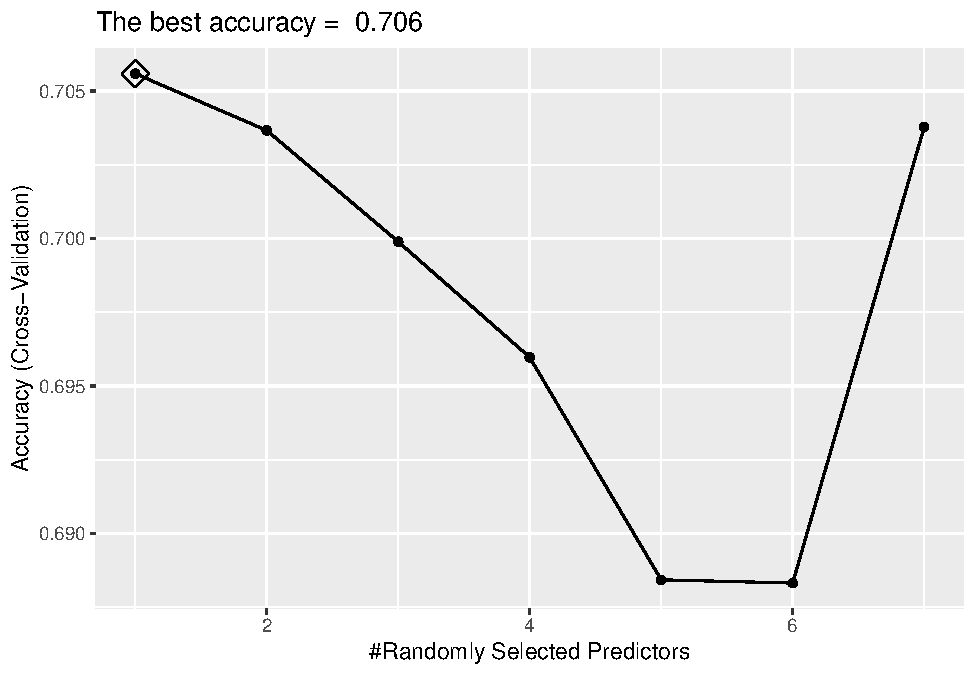
\includegraphics{LiverDisease_files/figure-latex/unnamed-chunk-35-1.pdf}

\begin{Shaded}
\begin{Highlighting}[]
\CommentTok{# Storing the results}
\NormalTok{model_results <-}\StringTok{ }\KeywordTok{bind_rows}\NormalTok{(model_results,}\KeywordTok{data_frame}\NormalTok{(}\DataTypeTok{method=}\StringTok{"rf_pca"}\NormalTok{,  }
                                     \DataTypeTok{Accuracy =} \KeywordTok{max}\NormalTok{(train_rf_pca}\OperatorTok{$}\NormalTok{results}\OperatorTok{$}\NormalTok{Accuracy) ))}
\end{Highlighting}
\end{Shaded}

The reported accuracies and kappas for all models across the training
dataset are shown in the following table and graph. The results show
that \emph{qda} model performs the worse. All other models provide an
accuracy of around 0.70. The random forest, along with the principal
component analysis, gives the best performance.

\begin{Shaded}
\begin{Highlighting}[]
\NormalTok{model_results}
\end{Highlighting}
\end{Shaded}

\begin{longtable}[]{@{}lr@{}}
\toprule
method & Accuracy\tabularnewline
\midrule
\endhead
glm & 0.7024949\tabularnewline
knn & 0.7002355\tabularnewline
loess & 0.6956271\tabularnewline
pls & 0.7143429\tabularnewline
lda & 0.7101339\tabularnewline
qda & 0.5571708\tabularnewline
rpart & 0.7150976\tabularnewline
rf & 0.7063528\tabularnewline
svm & 0.7150976\tabularnewline
ada & 0.7135809\tabularnewline
rf\_pca & 0.7108886\tabularnewline
\bottomrule
\end{longtable}

\begin{Shaded}
\begin{Highlighting}[]
\CommentTok{# collect resamples}
\NormalTok{results <-}\StringTok{ }\KeywordTok{resamples}\NormalTok{(}\KeywordTok{list}\NormalTok{(}\DataTypeTok{GLM=}\NormalTok{train_glm, }
                          \DataTypeTok{KNN =}\NormalTok{ train_knn,}
                          \DataTypeTok{LOESS=}\NormalTok{train_loess,}
                          \DataTypeTok{PLS=}\NormalTok{ train_pls,}
                          \DataTypeTok{LDA =}\NormalTok{ train_lda,}
                          \DataTypeTok{QDA =}\NormalTok{ train_qda,}
                          \DataTypeTok{RPART =}\NormalTok{ train_rpart,}
                          \DataTypeTok{RF =}\NormalTok{ train_rf,}
                          \DataTypeTok{SVM =}\NormalTok{ train_svm,}
                          \DataTypeTok{ADA=}\NormalTok{ train_ada,}
                          \DataTypeTok{RF_PCA =}\NormalTok{ train_rf_pca))}
\CommentTok{# boxplots of results}
\KeywordTok{bwplot}\NormalTok{(results)}
\end{Highlighting}
\end{Shaded}

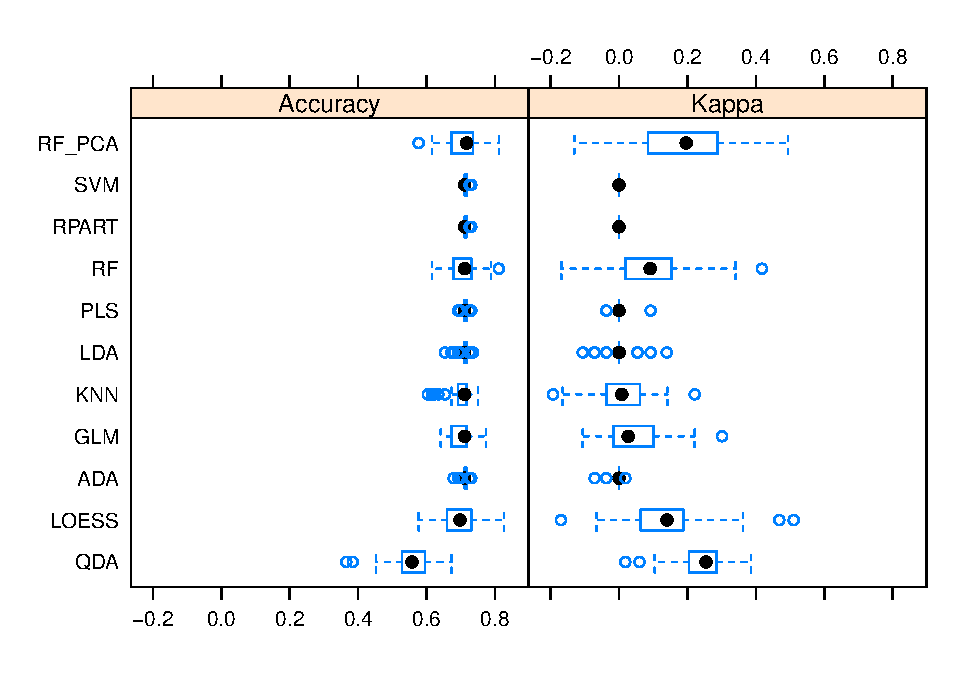
\includegraphics{LiverDisease_files/figure-latex/unnamed-chunk-37-1.pdf}

\section{Results}
\label{sec:results}

The statistical measurements of accuracy and precision reveal the
necessary reliability of a test. Specificity is the ability of a test to
exclude individuals who do not have a given disease correctly, and
sensitivity is the ability of a test to identify people who have a given
disease accurately. On the other hand, the F1 score is the harmonic mean
of Precision and Recall and gives a better measure of the incorrectly
classified cases than the accuracy metric. And, the kappa metric
measures the inter-rater reliability.

In Section \ref{sec:methods}, we trained several models using training
data. Now, we will evaluate the performance of these models using
validation data. We have not used \textbf{qda} model due to poor
performance on training data. The results show that \textbf{rf} and
\textbackslash emph\{rf\_pca\} models performs best in terms of
precision and recall. However, the models have slightly lower
sensitivity and specificity compared to other models. But, the
\textbackslash textbf\{rf\_pca\} model gives the best kappa value and is
significantly better than the remaining ones. So, we can deduce that
overall, \textbackslash textbf\{rf\_pca\} performs the best compared to
other models.

\begin{Shaded}
\begin{Highlighting}[]
\CommentTok{# Function to display a confusion matrix}
\CommentTok{# Code Source:}
\CommentTok{# https://stackoverflow.com/questions/23891140/r-how-to-visualize-confusion-matrix-using-the-caret-package}

\NormalTok{draw_confusion_matrix <-}\StringTok{ }\ControlFlowTok{function}\NormalTok{(cm, title) \{}

\NormalTok{  total <-}\StringTok{ }\KeywordTok{sum}\NormalTok{(cm}\OperatorTok{$}\NormalTok{table)}
\NormalTok{  res <-}\StringTok{ }\KeywordTok{as.numeric}\NormalTok{(cm}\OperatorTok{$}\NormalTok{table)}

  \CommentTok{# Generate color gradients. Palettes come from RColorBrewer.}
\NormalTok{  greenPalette <-}\StringTok{ }\KeywordTok{c}\NormalTok{(}\StringTok{"#F7FCF5"}\NormalTok{,}\StringTok{"#E5F5E0"}\NormalTok{,}\StringTok{"#C7E9C0"}\NormalTok{,}\StringTok{"#A1D99B"}\NormalTok{,}\StringTok{"#74C476"}\NormalTok{,}\StringTok{"#41AB5D"}\NormalTok{,}\StringTok{"#238B45"}\NormalTok{,}\StringTok{"#006D2C"}\NormalTok{,}\StringTok{"#00441B"}\NormalTok{)}
\NormalTok{  redPalette <-}\StringTok{ }\KeywordTok{c}\NormalTok{(}\StringTok{"#FFF5F0"}\NormalTok{,}\StringTok{"#FEE0D2"}\NormalTok{,}\StringTok{"#FCBBA1"}\NormalTok{,}\StringTok{"#FC9272"}\NormalTok{,}\StringTok{"#FB6A4A"}\NormalTok{,}\StringTok{"#EF3B2C"}\NormalTok{,}\StringTok{"#CB181D"}\NormalTok{,}\StringTok{"#A50F15"}\NormalTok{,}\StringTok{"#67000D"}\NormalTok{)}
\NormalTok{  getColor <-}\StringTok{ }\ControlFlowTok{function}\NormalTok{ (}\DataTypeTok{greenOrRed =} \StringTok{"green"}\NormalTok{, }\DataTypeTok{amount =} \DecValTok{0}\NormalTok{) \{}
    \ControlFlowTok{if}\NormalTok{ (amount }\OperatorTok{==}\StringTok{ }\DecValTok{0}\NormalTok{)}
      \KeywordTok{return}\NormalTok{(}\StringTok{"#FFFFFF"}\NormalTok{)}
\NormalTok{    palette <-}\StringTok{ }\NormalTok{greenPalette}
    \ControlFlowTok{if}\NormalTok{ (greenOrRed }\OperatorTok{==}\StringTok{ "red"}\NormalTok{)}
\NormalTok{      palette <-}\StringTok{ }\NormalTok{redPalette}
    \KeywordTok{colorRampPalette}\NormalTok{(palette)(}\DecValTok{100}\NormalTok{)[}\DecValTok{10} \OperatorTok{+}\StringTok{ }\KeywordTok{ceiling}\NormalTok{(}\DecValTok{90} \OperatorTok{*}\StringTok{ }\NormalTok{amount }\OperatorTok{/}\StringTok{ }\NormalTok{total)]}
\NormalTok{  \}}

  \CommentTok{# set the basic layout}
  \KeywordTok{layout}\NormalTok{(}\KeywordTok{matrix}\NormalTok{(}\KeywordTok{c}\NormalTok{(}\DecValTok{1}\NormalTok{,}\DecValTok{1}\NormalTok{,}\DecValTok{2}\NormalTok{)))}
  \KeywordTok{par}\NormalTok{(}\DataTypeTok{mar=}\KeywordTok{c}\NormalTok{(}\DecValTok{2}\NormalTok{,}\DecValTok{2}\NormalTok{,}\DecValTok{2}\NormalTok{,}\DecValTok{2}\NormalTok{))}
  \KeywordTok{plot}\NormalTok{(}\KeywordTok{c}\NormalTok{(}\DecValTok{100}\NormalTok{, }\DecValTok{345}\NormalTok{), }\KeywordTok{c}\NormalTok{(}\DecValTok{300}\NormalTok{, }\DecValTok{450}\NormalTok{), }\DataTypeTok{type =} \StringTok{"n"}\NormalTok{, }\DataTypeTok{xlab=}\StringTok{""}\NormalTok{, }\DataTypeTok{ylab=}\StringTok{""}\NormalTok{, }\DataTypeTok{xaxt=}\StringTok{'n'}\NormalTok{, }\DataTypeTok{yaxt=}\StringTok{'n'}\NormalTok{)}
  \KeywordTok{title}\NormalTok{(title, }\DataTypeTok{cex.main=}\DecValTok{2}\NormalTok{)}

  \CommentTok{# create the matrix }
\NormalTok{  classes =}\StringTok{ }\KeywordTok{colnames}\NormalTok{(cm}\OperatorTok{$}\NormalTok{table)}
  \KeywordTok{rect}\NormalTok{(}\DecValTok{150}\NormalTok{, }\DecValTok{430}\NormalTok{, }\DecValTok{240}\NormalTok{, }\DecValTok{370}\NormalTok{, }\DataTypeTok{col=}\KeywordTok{getColor}\NormalTok{(}\StringTok{"green"}\NormalTok{, res[}\DecValTok{1}\NormalTok{]))}
  \KeywordTok{text}\NormalTok{(}\DecValTok{195}\NormalTok{, }\DecValTok{435}\NormalTok{, classes[}\DecValTok{1}\NormalTok{], }\DataTypeTok{cex=}\FloatTok{1.2}\NormalTok{)}
  \KeywordTok{rect}\NormalTok{(}\DecValTok{250}\NormalTok{, }\DecValTok{430}\NormalTok{, }\DecValTok{340}\NormalTok{, }\DecValTok{370}\NormalTok{, }\DataTypeTok{col=}\KeywordTok{getColor}\NormalTok{(}\StringTok{"red"}\NormalTok{, res[}\DecValTok{3}\NormalTok{]))}
  \KeywordTok{text}\NormalTok{(}\DecValTok{295}\NormalTok{, }\DecValTok{435}\NormalTok{, classes[}\DecValTok{2}\NormalTok{], }\DataTypeTok{cex=}\FloatTok{1.2}\NormalTok{)}
  \KeywordTok{text}\NormalTok{(}\DecValTok{125}\NormalTok{, }\DecValTok{370}\NormalTok{, }\StringTok{'Predicted'}\NormalTok{, }\DataTypeTok{cex=}\FloatTok{1.3}\NormalTok{, }\DataTypeTok{srt=}\DecValTok{90}\NormalTok{, }\DataTypeTok{font=}\DecValTok{2}\NormalTok{)}
  \KeywordTok{text}\NormalTok{(}\DecValTok{245}\NormalTok{, }\DecValTok{450}\NormalTok{, }\StringTok{'Actual'}\NormalTok{, }\DataTypeTok{cex=}\FloatTok{1.3}\NormalTok{, }\DataTypeTok{font=}\DecValTok{2}\NormalTok{)}
  \KeywordTok{rect}\NormalTok{(}\DecValTok{150}\NormalTok{, }\DecValTok{305}\NormalTok{, }\DecValTok{240}\NormalTok{, }\DecValTok{365}\NormalTok{, }\DataTypeTok{col=}\KeywordTok{getColor}\NormalTok{(}\StringTok{"red"}\NormalTok{, res[}\DecValTok{2}\NormalTok{]))}
  \KeywordTok{rect}\NormalTok{(}\DecValTok{250}\NormalTok{, }\DecValTok{305}\NormalTok{, }\DecValTok{340}\NormalTok{, }\DecValTok{365}\NormalTok{, }\DataTypeTok{col=}\KeywordTok{getColor}\NormalTok{(}\StringTok{"green"}\NormalTok{, res[}\DecValTok{4}\NormalTok{]))}
  \KeywordTok{text}\NormalTok{(}\DecValTok{140}\NormalTok{, }\DecValTok{400}\NormalTok{, classes[}\DecValTok{1}\NormalTok{], }\DataTypeTok{cex=}\FloatTok{1.2}\NormalTok{, }\DataTypeTok{srt=}\DecValTok{90}\NormalTok{)}
  \KeywordTok{text}\NormalTok{(}\DecValTok{140}\NormalTok{, }\DecValTok{335}\NormalTok{, classes[}\DecValTok{2}\NormalTok{], }\DataTypeTok{cex=}\FloatTok{1.2}\NormalTok{, }\DataTypeTok{srt=}\DecValTok{90}\NormalTok{)}

  \CommentTok{# add in the cm results}
  \KeywordTok{text}\NormalTok{(}\DecValTok{195}\NormalTok{, }\DecValTok{400}\NormalTok{, res[}\DecValTok{1}\NormalTok{], }\DataTypeTok{cex=}\FloatTok{1.6}\NormalTok{, }\DataTypeTok{font=}\DecValTok{2}\NormalTok{, }\DataTypeTok{col=}\StringTok{'white'}\NormalTok{)}
  \KeywordTok{text}\NormalTok{(}\DecValTok{195}\NormalTok{, }\DecValTok{335}\NormalTok{, res[}\DecValTok{2}\NormalTok{], }\DataTypeTok{cex=}\FloatTok{1.6}\NormalTok{, }\DataTypeTok{font=}\DecValTok{2}\NormalTok{, }\DataTypeTok{col=}\StringTok{'white'}\NormalTok{)}
  \KeywordTok{text}\NormalTok{(}\DecValTok{295}\NormalTok{, }\DecValTok{400}\NormalTok{, res[}\DecValTok{3}\NormalTok{], }\DataTypeTok{cex=}\FloatTok{1.6}\NormalTok{, }\DataTypeTok{font=}\DecValTok{2}\NormalTok{, }\DataTypeTok{col=}\StringTok{'white'}\NormalTok{)}
  \KeywordTok{text}\NormalTok{(}\DecValTok{295}\NormalTok{, }\DecValTok{335}\NormalTok{, res[}\DecValTok{4}\NormalTok{], }\DataTypeTok{cex=}\FloatTok{1.6}\NormalTok{, }\DataTypeTok{font=}\DecValTok{2}\NormalTok{, }\DataTypeTok{col=}\StringTok{'white'}\NormalTok{)}

  \CommentTok{# add in the specifics }
  \KeywordTok{plot}\NormalTok{(}\KeywordTok{c}\NormalTok{(}\DecValTok{100}\NormalTok{, }\DecValTok{0}\NormalTok{), }\KeywordTok{c}\NormalTok{(}\DecValTok{100}\NormalTok{, }\DecValTok{0}\NormalTok{), }\DataTypeTok{type =} \StringTok{"n"}\NormalTok{, }\DataTypeTok{xlab=}\StringTok{""}\NormalTok{, }\DataTypeTok{ylab=}\StringTok{""}\NormalTok{, }\DataTypeTok{main =} \StringTok{"DETAILS"}\NormalTok{, }\DataTypeTok{xaxt=}\StringTok{'n'}\NormalTok{, }\DataTypeTok{yaxt=}\StringTok{'n'}\NormalTok{)}
  \KeywordTok{text}\NormalTok{(}\DecValTok{10}\NormalTok{, }\DecValTok{85}\NormalTok{, }\KeywordTok{names}\NormalTok{(cm}\OperatorTok{$}\NormalTok{byClass[}\DecValTok{1}\NormalTok{]), }\DataTypeTok{cex=}\FloatTok{1.2}\NormalTok{, }\DataTypeTok{font=}\DecValTok{2}\NormalTok{)}
  \KeywordTok{text}\NormalTok{(}\DecValTok{10}\NormalTok{, }\DecValTok{70}\NormalTok{, }\KeywordTok{round}\NormalTok{(}\KeywordTok{as.numeric}\NormalTok{(cm}\OperatorTok{$}\NormalTok{byClass[}\DecValTok{1}\NormalTok{]), }\DecValTok{3}\NormalTok{), }\DataTypeTok{cex=}\FloatTok{1.2}\NormalTok{)}
  \KeywordTok{text}\NormalTok{(}\DecValTok{30}\NormalTok{, }\DecValTok{85}\NormalTok{, }\KeywordTok{names}\NormalTok{(cm}\OperatorTok{$}\NormalTok{byClass[}\DecValTok{2}\NormalTok{]), }\DataTypeTok{cex=}\FloatTok{1.2}\NormalTok{, }\DataTypeTok{font=}\DecValTok{2}\NormalTok{)}
  \KeywordTok{text}\NormalTok{(}\DecValTok{30}\NormalTok{, }\DecValTok{70}\NormalTok{, }\KeywordTok{round}\NormalTok{(}\KeywordTok{as.numeric}\NormalTok{(cm}\OperatorTok{$}\NormalTok{byClass[}\DecValTok{2}\NormalTok{]), }\DecValTok{3}\NormalTok{), }\DataTypeTok{cex=}\FloatTok{1.2}\NormalTok{)}
  \KeywordTok{text}\NormalTok{(}\DecValTok{50}\NormalTok{, }\DecValTok{85}\NormalTok{, }\KeywordTok{names}\NormalTok{(cm}\OperatorTok{$}\NormalTok{byClass[}\DecValTok{5}\NormalTok{]), }\DataTypeTok{cex=}\FloatTok{1.2}\NormalTok{, }\DataTypeTok{font=}\DecValTok{2}\NormalTok{)}
  \KeywordTok{text}\NormalTok{(}\DecValTok{50}\NormalTok{, }\DecValTok{70}\NormalTok{, }\KeywordTok{round}\NormalTok{(}\KeywordTok{as.numeric}\NormalTok{(cm}\OperatorTok{$}\NormalTok{byClass[}\DecValTok{5}\NormalTok{]), }\DecValTok{3}\NormalTok{), }\DataTypeTok{cex=}\FloatTok{1.2}\NormalTok{)}
  \KeywordTok{text}\NormalTok{(}\DecValTok{70}\NormalTok{, }\DecValTok{85}\NormalTok{, }\KeywordTok{names}\NormalTok{(cm}\OperatorTok{$}\NormalTok{byClass[}\DecValTok{6}\NormalTok{]), }\DataTypeTok{cex=}\FloatTok{1.2}\NormalTok{, }\DataTypeTok{font=}\DecValTok{2}\NormalTok{)}
  \KeywordTok{text}\NormalTok{(}\DecValTok{70}\NormalTok{, }\DecValTok{70}\NormalTok{, }\KeywordTok{round}\NormalTok{(}\KeywordTok{as.numeric}\NormalTok{(cm}\OperatorTok{$}\NormalTok{byClass[}\DecValTok{6}\NormalTok{]), }\DecValTok{3}\NormalTok{), }\DataTypeTok{cex=}\FloatTok{1.2}\NormalTok{)}
  \KeywordTok{text}\NormalTok{(}\DecValTok{90}\NormalTok{, }\DecValTok{85}\NormalTok{, }\KeywordTok{names}\NormalTok{(cm}\OperatorTok{$}\NormalTok{byClass[}\DecValTok{7}\NormalTok{]), }\DataTypeTok{cex=}\FloatTok{1.2}\NormalTok{, }\DataTypeTok{font=}\DecValTok{2}\NormalTok{)}
  \KeywordTok{text}\NormalTok{(}\DecValTok{90}\NormalTok{, }\DecValTok{70}\NormalTok{, }\KeywordTok{round}\NormalTok{(}\KeywordTok{as.numeric}\NormalTok{(cm}\OperatorTok{$}\NormalTok{byClass[}\DecValTok{7}\NormalTok{]), }\DecValTok{3}\NormalTok{), }\DataTypeTok{cex=}\FloatTok{1.2}\NormalTok{)}
 
  \CommentTok{# add in the accuracy information }
  \KeywordTok{text}\NormalTok{(}\DecValTok{30}\NormalTok{, }\DecValTok{35}\NormalTok{, }\KeywordTok{names}\NormalTok{(cm}\OperatorTok{$}\NormalTok{overall[}\DecValTok{1}\NormalTok{]), }\DataTypeTok{cex=}\FloatTok{1.5}\NormalTok{, }\DataTypeTok{font=}\DecValTok{2}\NormalTok{)}
  \KeywordTok{text}\NormalTok{(}\DecValTok{30}\NormalTok{, }\DecValTok{20}\NormalTok{, }\KeywordTok{round}\NormalTok{(}\KeywordTok{as.numeric}\NormalTok{(cm}\OperatorTok{$}\NormalTok{overall[}\DecValTok{1}\NormalTok{]), }\DecValTok{3}\NormalTok{), }\DataTypeTok{cex=}\FloatTok{1.4}\NormalTok{)}
  \KeywordTok{text}\NormalTok{(}\DecValTok{70}\NormalTok{, }\DecValTok{35}\NormalTok{, }\KeywordTok{names}\NormalTok{(cm}\OperatorTok{$}\NormalTok{overall[}\DecValTok{2}\NormalTok{]), }\DataTypeTok{cex=}\FloatTok{1.5}\NormalTok{, }\DataTypeTok{font=}\DecValTok{2}\NormalTok{)}
  \KeywordTok{text}\NormalTok{(}\DecValTok{70}\NormalTok{, }\DecValTok{20}\NormalTok{, }\KeywordTok{round}\NormalTok{(}\KeywordTok{as.numeric}\NormalTok{(cm}\OperatorTok{$}\NormalTok{overall[}\DecValTok{2}\NormalTok{]), }\DecValTok{3}\NormalTok{), }\DataTypeTok{cex=}\FloatTok{1.4}\NormalTok{)}
\NormalTok{\}}
\end{Highlighting}
\end{Shaded}

\begin{Shaded}
\begin{Highlighting}[]
\CommentTok{# Creating an empty data frame to hold the results of models }
\CommentTok{# across validation dataset}
\NormalTok{ml_results<-}\KeywordTok{data_frame}\NormalTok{()}

\CommentTok{# Function to compute all stats from models}
\NormalTok{evaluate_performance <-}\StringTok{ }\ControlFlowTok{function}\NormalTok{(model_name, model, validation,model_results,title) }
\NormalTok{\{}
  \CommentTok{# Generating predictions}
\NormalTok{  predictions<-}\KeywordTok{predict}\NormalTok{(model, validation)}
  
   \CommentTok{# Draw the confusion matrix}
\NormalTok{  cm<-}\KeywordTok{confusionMatrix}\NormalTok{(predictions,validation}\OperatorTok{$}\NormalTok{LiverDisease,}\DataTypeTok{positive=}\StringTok{"M"}\NormalTok{)}
  
  \KeywordTok{draw_confusion_matrix}\NormalTok{(cm,title)}
 
  \CommentTok{# Generate metrics}
\NormalTok{  sensitivty<-}\KeywordTok{as.numeric}\NormalTok{(cm}\OperatorTok{$}\NormalTok{byClass[}\DecValTok{1}\NormalTok{])}
\NormalTok{  specificity<-}\KeywordTok{as.numeric}\NormalTok{(cm}\OperatorTok{$}\NormalTok{byClass[}\DecValTok{2}\NormalTok{])}
\NormalTok{  precision<-}\KeywordTok{as.numeric}\NormalTok{(cm}\OperatorTok{$}\NormalTok{byClass[}\DecValTok{5}\NormalTok{])}
\NormalTok{  recall<-}\KeywordTok{as.numeric}\NormalTok{(cm}\OperatorTok{$}\NormalTok{byClass[}\DecValTok{6}\NormalTok{])}
\NormalTok{  f1_score<-}\KeywordTok{as.numeric}\NormalTok{(cm}\OperatorTok{$}\NormalTok{byClass[}\DecValTok{7}\NormalTok{])}
\NormalTok{  accuracy<-}\KeywordTok{as.numeric}\NormalTok{(cm}\OperatorTok{$}\NormalTok{overall[}\DecValTok{1}\NormalTok{])}
\NormalTok{  kappa <-}\KeywordTok{as.numeric}\NormalTok{(cm}\OperatorTok{$}\NormalTok{overall[}\DecValTok{2}\NormalTok{])}
  
  \CommentTok{# Store metrics to a data frame}
\NormalTok{  ml_results <-}\StringTok{ }\KeywordTok{bind_rows}\NormalTok{(ml_results, }\KeywordTok{data_frame}\NormalTok{(}\DataTypeTok{Models =}\NormalTok{ model_name,}
             \DataTypeTok{Accuracy =}\NormalTok{ accuracy,}
             \DataTypeTok{Precision=}\NormalTok{ precision,}
             \DataTypeTok{Sensitivty=}\NormalTok{sensitivty,}
             \DataTypeTok{Specificity=}\NormalTok{specificity,}
             \DataTypeTok{F1_Score =}\NormalTok{ f1_score,}
             \DataTypeTok{Kappa=}\NormalTok{ kappa))}
\NormalTok{\}}

\CommentTok{# Evaluating the performance of models}
\NormalTok{ml_results<-}\KeywordTok{evaluate_performance}\NormalTok{(}\StringTok{"glm"}\NormalTok{,train_glm,validation,ml_results,}\StringTok{"Confusion Matrix - glm"}\NormalTok{)}
\end{Highlighting}
\end{Shaded}

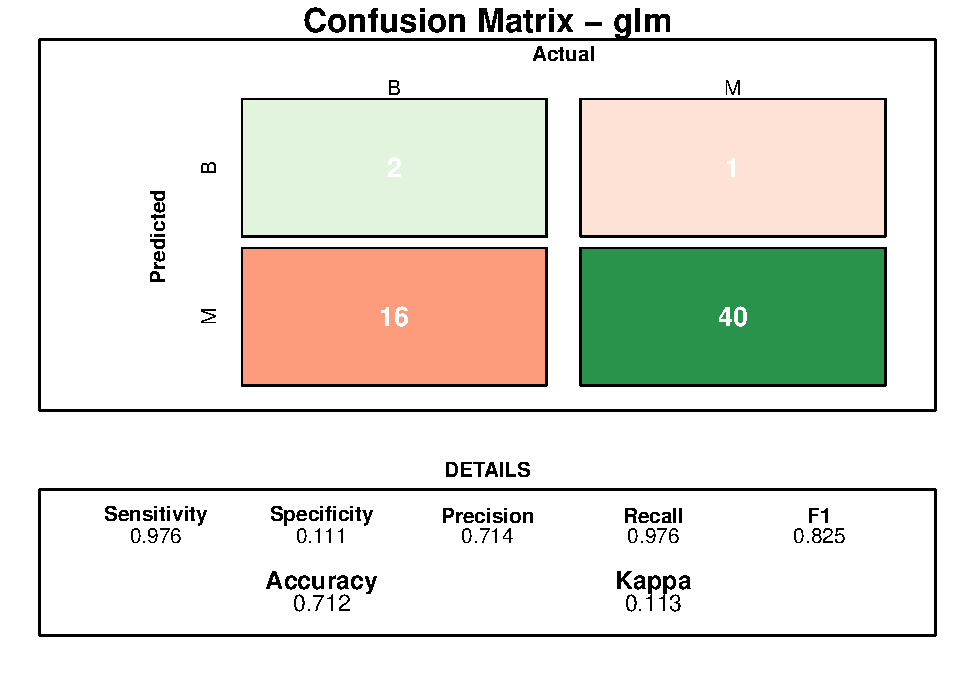
\includegraphics{LiverDisease_files/figure-latex/unnamed-chunk-39-1.pdf}

\begin{Shaded}
\begin{Highlighting}[]
\CommentTok{# Evaluate knn model}
\NormalTok{ml_results<-}\KeywordTok{evaluate_performance}\NormalTok{(}\StringTok{"knn"}\NormalTok{,train_knn,validation,ml_results,}\StringTok{"Confusion Matrix - knn"}\NormalTok{)}
\end{Highlighting}
\end{Shaded}

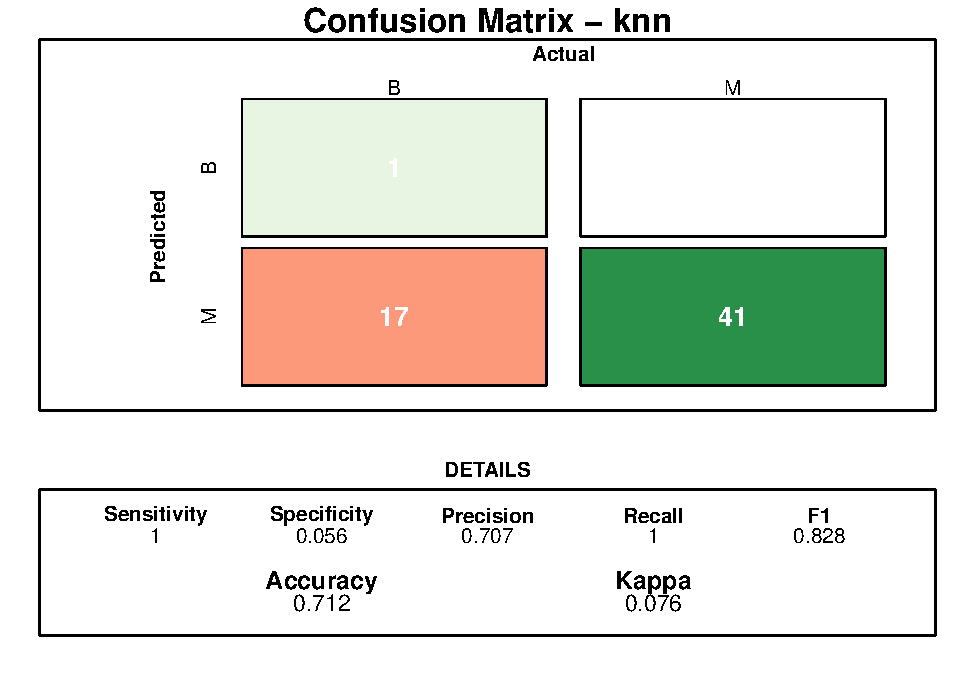
\includegraphics{LiverDisease_files/figure-latex/unnamed-chunk-40-1.pdf}

\begin{Shaded}
\begin{Highlighting}[]
\CommentTok{#Evaluate loess model}
\NormalTok{ml_results<-}\KeywordTok{evaluate_performance}\NormalTok{(}\StringTok{"loess"}\NormalTok{,train_loess,validation,ml_results,}\StringTok{"Confusion Matrix - loess"}\NormalTok{)}
\end{Highlighting}
\end{Shaded}

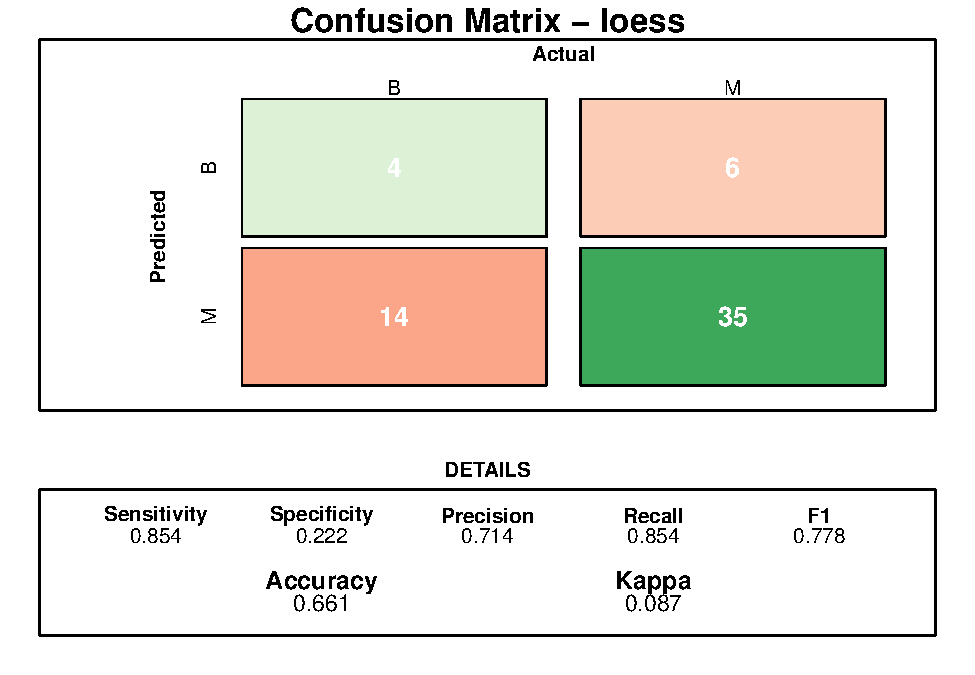
\includegraphics{LiverDisease_files/figure-latex/unnamed-chunk-41-1.pdf}

\begin{Shaded}
\begin{Highlighting}[]
\NormalTok{ml_results<-}\KeywordTok{evaluate_performance}\NormalTok{(}\StringTok{"pls"}\NormalTok{,train_pls,validation,ml_results,}\StringTok{"Confusion Matrix -pls"}\NormalTok{)}
\end{Highlighting}
\end{Shaded}

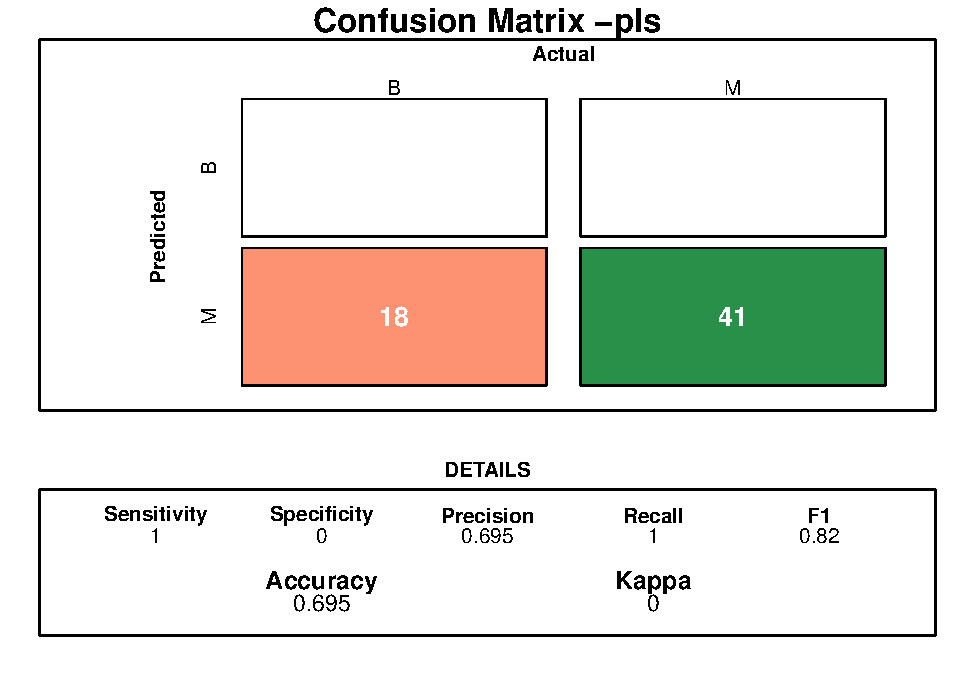
\includegraphics{LiverDisease_files/figure-latex/unnamed-chunk-42-1.pdf}

\begin{Shaded}
\begin{Highlighting}[]
\NormalTok{ml_results<-}\KeywordTok{evaluate_performance}\NormalTok{(}\StringTok{"lda"}\NormalTok{,train_lda,validation,ml_results, }\StringTok{"Confusion Matrix - lda"}\NormalTok{)}
\end{Highlighting}
\end{Shaded}

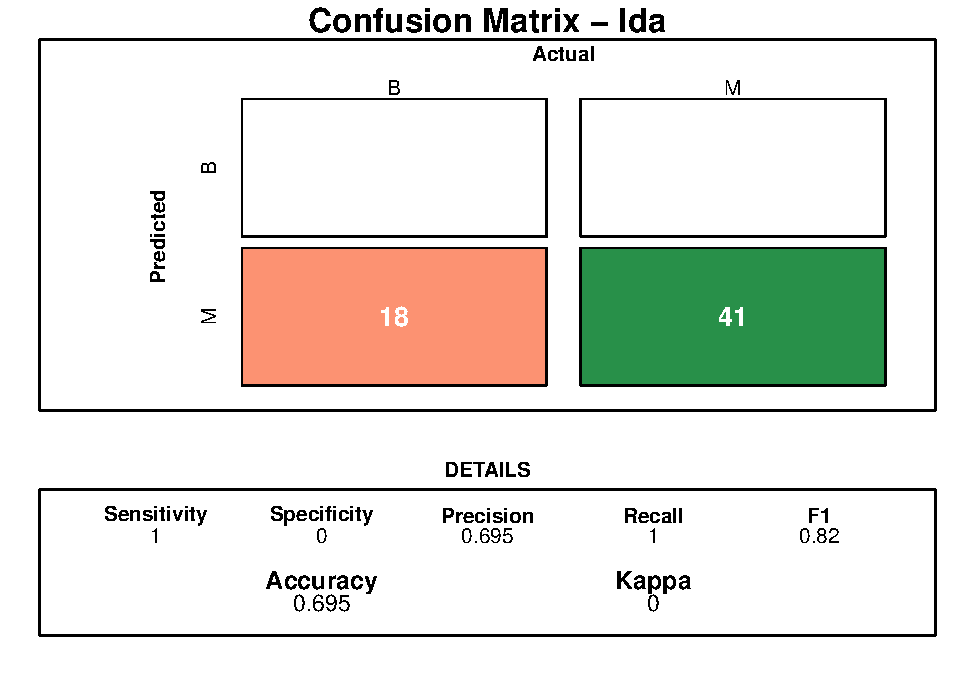
\includegraphics{LiverDisease_files/figure-latex/unnamed-chunk-43-1.pdf}

\begin{Shaded}
\begin{Highlighting}[]
\NormalTok{ml_results<-}\KeywordTok{evaluate_performance}\NormalTok{(}\StringTok{"rpart"}\NormalTok{,train_rpart,validation,ml_results, }\StringTok{"Confusion Matrix - rpart"}\NormalTok{)}
\end{Highlighting}
\end{Shaded}

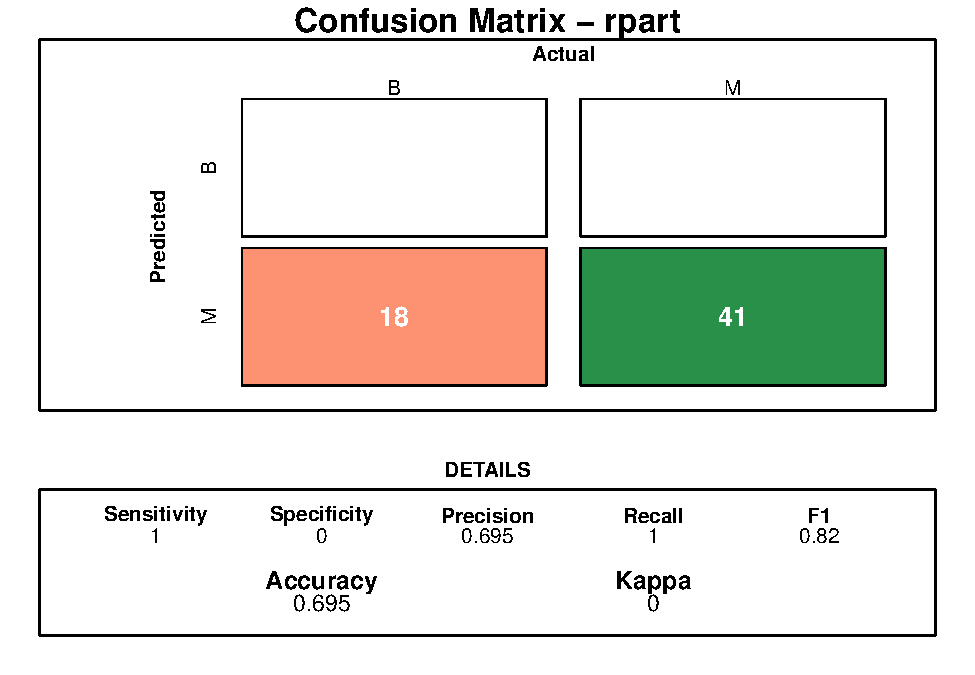
\includegraphics{LiverDisease_files/figure-latex/unnamed-chunk-44-1.pdf}

\begin{Shaded}
\begin{Highlighting}[]
\NormalTok{ml_results<-}\KeywordTok{evaluate_performance}\NormalTok{(}\StringTok{"rf"}\NormalTok{,train_rf,validation,ml_results,}\StringTok{"Confusion Matrix - rf"}\NormalTok{)}
\end{Highlighting}
\end{Shaded}

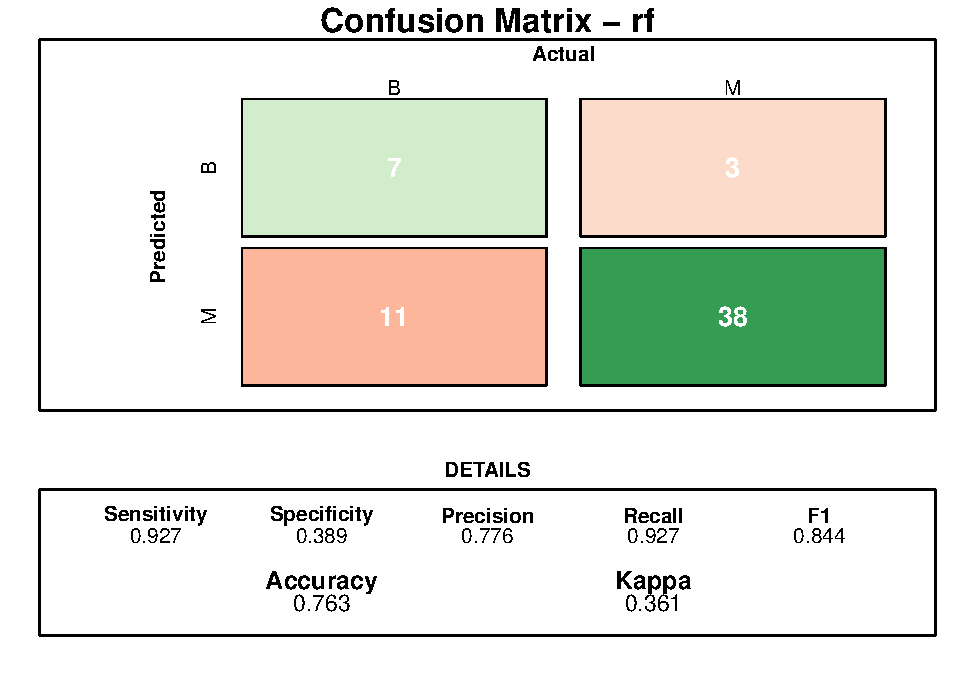
\includegraphics{LiverDisease_files/figure-latex/unnamed-chunk-45-1.pdf}

\begin{Shaded}
\begin{Highlighting}[]
\NormalTok{ml_results<-}\KeywordTok{evaluate_performance}\NormalTok{(}\StringTok{"svmlinear"}\NormalTok{,train_svm,validation,ml_results, }\StringTok{"Confusion Matrix - svm"}\NormalTok{)}
\end{Highlighting}
\end{Shaded}

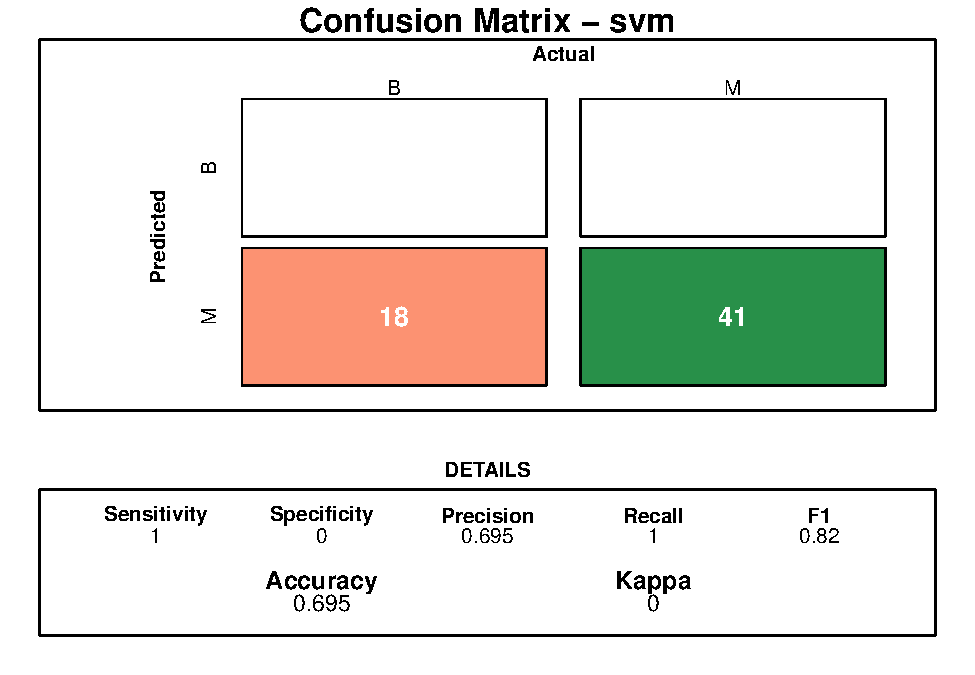
\includegraphics{LiverDisease_files/figure-latex/unnamed-chunk-46-1.pdf}

\begin{Shaded}
\begin{Highlighting}[]
\NormalTok{ml_results<-}\KeywordTok{evaluate_performance}\NormalTok{(}\StringTok{"ada"}\NormalTok{,train_ada,validation,ml_results,}\StringTok{"Confusion Matrix - adaboost"}\NormalTok{)}
\end{Highlighting}
\end{Shaded}

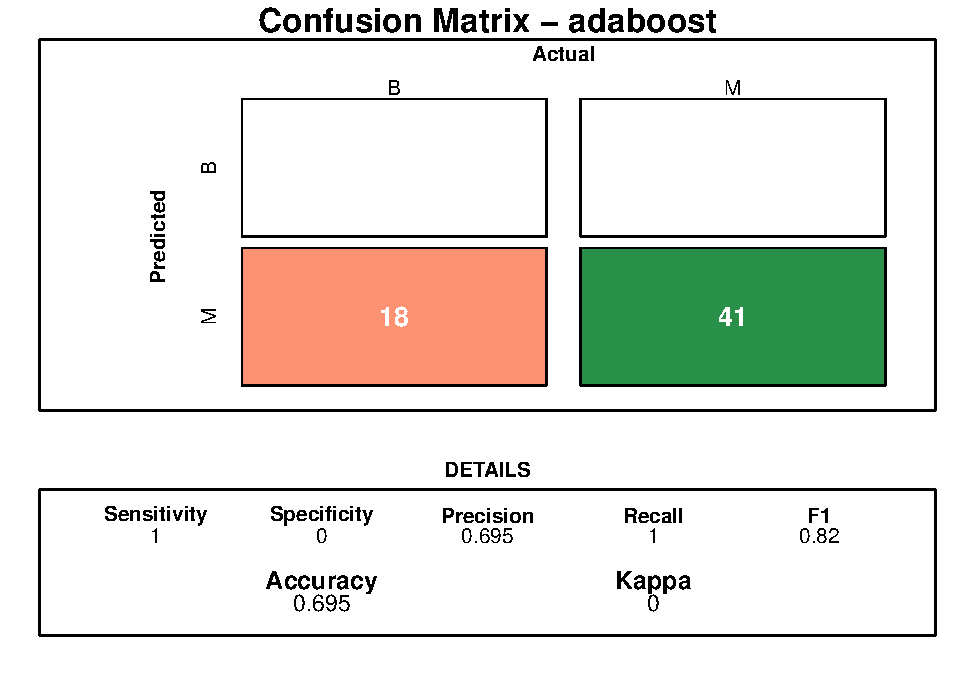
\includegraphics{LiverDisease_files/figure-latex/unnamed-chunk-47-1.pdf}

\begin{Shaded}
\begin{Highlighting}[]
\NormalTok{ml_results<-}\KeywordTok{evaluate_performance}\NormalTok{(}\StringTok{"rf_pca"}\NormalTok{,train_rf_pca,validation,ml_results,}\StringTok{"Confusion Matrix - rf pca"}\NormalTok{)}
\end{Highlighting}
\end{Shaded}

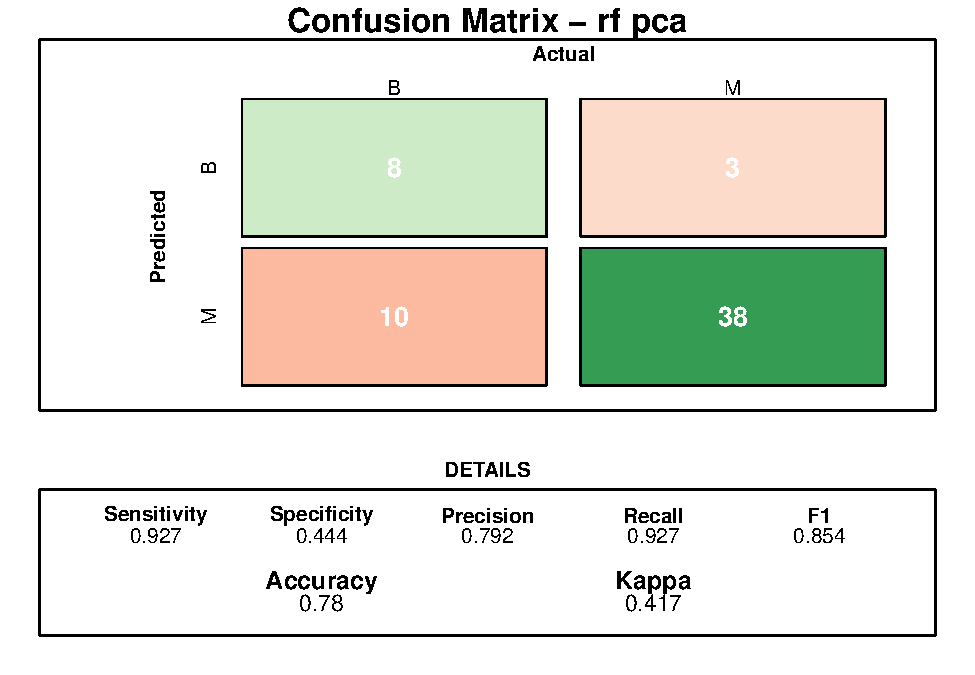
\includegraphics{LiverDisease_files/figure-latex/unnamed-chunk-48-1.pdf}

Now, we do an experiment to combine the predictions of multiple models,
i.e., ensemble model. The idea is to diagnose a liver disease only if
50\% of the predictions from different models vote that the liver has a
disease. The accuracy of the model and the resulting confusion matrix is
not good to consider it for further analysis.

\begin{Shaded}
\begin{Highlighting}[]
\CommentTok{# Generating prediction of all models}
\NormalTok{glm_predictions<-}\KeywordTok{predict}\NormalTok{(train_glm, validation)}
\NormalTok{knn_predictions<-}\KeywordTok{predict}\NormalTok{(train_knn, validation)}
\NormalTok{loess_predictions<-}\KeywordTok{predict}\NormalTok{(train_loess, validation)}
\NormalTok{pls_predictions<-}\KeywordTok{predict}\NormalTok{(train_pls, validation)}
\NormalTok{lda_predictions<-}\KeywordTok{predict}\NormalTok{(train_lda, validation)}
\NormalTok{rpart_predictions<-}\KeywordTok{predict}\NormalTok{(train_rpart, validation)}
\NormalTok{rf_predictions<-}\KeywordTok{predict}\NormalTok{(train_rf, validation)}
\NormalTok{svmlinear_predictions<-}\KeywordTok{predict}\NormalTok{(train_svm, validation)}
\NormalTok{ada_predictions<-}\KeywordTok{predict}\NormalTok{(train_ada, validation)}
\NormalTok{rf_pca_predictions<-}\KeywordTok{predict}\NormalTok{(train_rf_pca, validation)}

\CommentTok{# Generate outputs fpr ensemble model}
\NormalTok{ensemble_pred<-}\KeywordTok{data.frame}\NormalTok{(glm_predictions, }
\NormalTok{                          knn_predictions,}
\NormalTok{                          loess_predictions,}
\NormalTok{                          pls_predictions, }
\NormalTok{                          lda_predictions,}
\NormalTok{                          rpart_predictions, }
\NormalTok{                          rf_predictions, }
\NormalTok{                          svmlinear_predictions,}
\NormalTok{                          ada_predictions,}
\NormalTok{                          rf_pca_predictions)}

\CommentTok{# If 50% of the predictions say disease then we pick it a disease}
\NormalTok{votes <-}\StringTok{ }\KeywordTok{rowMeans}\NormalTok{(ensemble_pred}\OperatorTok{==}\StringTok{"M"}\NormalTok{)}
\NormalTok{ensemble_predictions <-}\StringTok{ }\KeywordTok{ifelse}\NormalTok{(votes }\OperatorTok{>}\StringTok{ }\FloatTok{0.5}\NormalTok{, }\StringTok{"M"}\NormalTok{, }\StringTok{"B"}\NormalTok{) }\OperatorTok\StringTok{ }\KeywordTok{factor}\NormalTok{()}

\CommentTok{# Generate metrics}
\NormalTok{cm<-}\KeywordTok{confusionMatrix}\NormalTok{(ensemble_predictions,validation}\OperatorTok{$}\NormalTok{LiverDisease,}\DataTypeTok{positive=}\StringTok{"M"}\NormalTok{)}
\KeywordTok{draw_confusion_matrix}\NormalTok{(cm,}\StringTok{"Confusion Matrix - ensemble"}\NormalTok{)}
\end{Highlighting}
\end{Shaded}

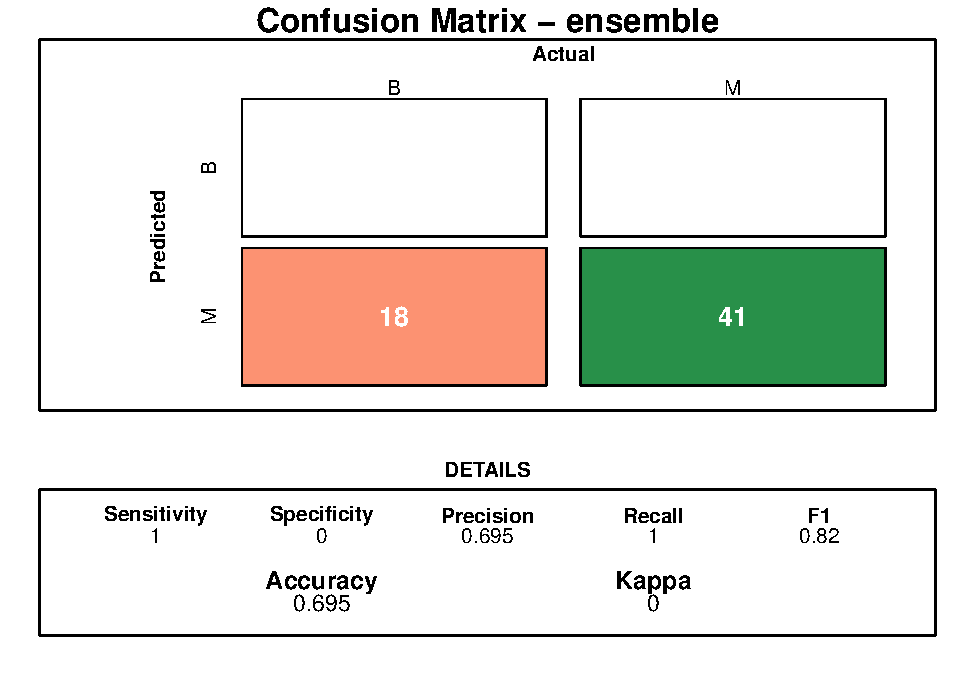
\includegraphics{LiverDisease_files/figure-latex/unnamed-chunk-49-1.pdf}

\begin{Shaded}
\begin{Highlighting}[]
\NormalTok{sensitivty<-}\KeywordTok{as.numeric}\NormalTok{(cm}\OperatorTok{$}\NormalTok{byClass[}\DecValTok{1}\NormalTok{])}
\NormalTok{specificity<-}\KeywordTok{as.numeric}\NormalTok{(cm}\OperatorTok{$}\NormalTok{byClass[}\DecValTok{2}\NormalTok{])}
\NormalTok{precision<-}\KeywordTok{as.numeric}\NormalTok{(cm}\OperatorTok{$}\NormalTok{byClass[}\DecValTok{5}\NormalTok{])}
\NormalTok{recall<-}\KeywordTok{as.numeric}\NormalTok{(cm}\OperatorTok{$}\NormalTok{byClass[}\DecValTok{6}\NormalTok{])}
\NormalTok{f1_score<-}\KeywordTok{as.numeric}\NormalTok{(cm}\OperatorTok{$}\NormalTok{byClass[}\DecValTok{7}\NormalTok{])}
\NormalTok{accuracy<-}\KeywordTok{as.numeric}\NormalTok{(cm}\OperatorTok{$}\NormalTok{overall[}\DecValTok{1}\NormalTok{])}
\NormalTok{kappa <-}\KeywordTok{as.numeric}\NormalTok{(cm}\OperatorTok{$}\NormalTok{overall[}\DecValTok{2}\NormalTok{])}

\CommentTok{# Store metrics to a data frame}
\NormalTok{ml_results <-}\StringTok{ }\KeywordTok{bind_rows}\NormalTok{(ml_results, }\KeywordTok{data_frame}\NormalTok{(}\DataTypeTok{Models =} \StringTok{"Ensemble"}\NormalTok{,}
             \DataTypeTok{Accuracy =}\NormalTok{ accuracy,}
             \DataTypeTok{Precision=}\NormalTok{ precision,}
             \DataTypeTok{Sensitivty=}\NormalTok{sensitivty,}
             \DataTypeTok{Specificity=}\NormalTok{specificity,}
             \DataTypeTok{F1_Score =}\NormalTok{ f1_score,}
             \DataTypeTok{Kappa=}\NormalTok{ kappa))}
\end{Highlighting}
\end{Shaded}

From the results, we can see that \textbackslash emph\{rf\_pca\}
performs the best compared to the other models. We saw a significant
improvement in \emph{kappa} and \emph{Specifivity} measures compared to
the other models. Though, the model has a slightly lower sensitivity
compared to the other models.

\begin{Shaded}
\begin{Highlighting}[]
\NormalTok{ml_results}
\end{Highlighting}
\end{Shaded}

\begin{longtable}[]{@{}lrrrrrr@{}}
\toprule
Models & Accuracy & Precision & Sensitivty & Specificity & F1\_Score &
Kappa\tabularnewline
\midrule
\endhead
glm & 0.7118644 & 0.7142857 & 0.9756098 & 0.1111111 & 0.8247423 &
0.1131742\tabularnewline
knn & 0.7118644 & 0.7068966 & 1.0000000 & 0.0555556 & 0.8282828 &
0.0755760\tabularnewline
loess & 0.6610169 & 0.7142857 & 0.8536585 & 0.2222222 & 0.7777778 &
0.0866873\tabularnewline
pls & 0.6949153 & 0.6949153 & 1.0000000 & 0.0000000 & 0.8200000 &
0.0000000\tabularnewline
lda & 0.7118644 & 0.7068966 & 1.0000000 & 0.0555556 & 0.8282828 &
0.0755760\tabularnewline
rpart & 0.6949153 & 0.6949153 & 1.0000000 & 0.0000000 & 0.8200000 &
0.0000000\tabularnewline
rf & 0.7457627 & 0.7500000 & 0.9512195 & 0.2777778 & 0.8387097 &
0.2763696\tabularnewline
svmlinear & 0.6949153 & 0.6949153 & 1.0000000 & 0.0000000 & 0.8200000 &
0.0000000\tabularnewline
ada & 0.6949153 & 0.6949153 & 1.0000000 & 0.0000000 & 0.8200000 &
0.0000000\tabularnewline
rf\_pca & 0.7796610 & 0.7916667 & 0.9268293 & 0.4444444 & 0.8539326 &
0.4167300\tabularnewline
Ensemble & 0.6949153 & 0.6949153 & 1.0000000 & 0.0000000 & 0.8200000 &
0.0000000\tabularnewline
\bottomrule
\end{longtable}

\section{Conclusion}
\label{sec:conclusion}

In this project, we developed machine learning models to diagnose liver
disease by analysing protein levels in the blood. We used patients'
liver records collected from India. We found out that some variables did
not correlate with the presence or absence of liver disease. So, we
ignored those variables and used the remaining variables to train the
model.

The results show that \emph{rf+pca} performed the best on the validation
dataset. We tried to further improve the results by combining the
outputs of several models. The idea was to use votes to decide if the
liver has a disease. If more than 50\% of the models predict a disease,
then we consider that the liver is damaged. But, the resulting model did
not perform well.

All models seem to overfit the data, and we end up getting more
``Malignant'' cases. The \textbackslash emph\{rf\_pca\} performs better,
and we can correctly predict some ``Benign'' cases. The only reason we
can think of is data is imbalanced. Ideally, both classes should have an
equal distribution for patient records to train robust models. But, only
28\% of the data belong to patients with liver disease. That's why the
trained models are more biased in wrongly categorizing healthy patients.
The ideal solution is to get more data to produce robust models.
Alternatively, we can class weights to solve the problem of imbalanced
data. We will explore the concept of class weights in future work.

\begin{thebibliography}{9}
\bibitem{cad} 
Ethan Du-Crowa, Lucy Warrenb, Susan M Astleya and Johan Hullemanc,"Is there a safety-net effect with Computer-Aided Detection (CAD)?", Medical Imaging 2019.
\bibitem{ld}
Eugene, R., Sorrell, Michael F.; Maddrey, Willis C., "Schiff's Diseases of the Liver", 10th Edition, Lippincott Williams \& Wilkins by Schiff.

\bibitem{bendi}
Bendi,  Venkata . R, M. S. Prasad Babu, and N. B. Venkateswarlu, "Critical Comparative Study of Liver Patients from USA and INDIA: An Exploratory Analysis", International Journal of Computer Science Issues, May 2012.


\end{thebibliography}


\end{document}
